\documentclass[12pt]{beamer}
\usepackage{amsmath}
\usepackage{mathtools}
\usepackage{multimedia}
\usepackage{hyperref}
\usepackage{booktabs}

\usefonttheme{professionalfonts} % using non standard fonts for beamer
\usefonttheme{serif} % default family is serif
%\documentclass[12pt]{beamerthemeSam.sty}
\usepackage{epsf}
%\usepackage{pstricks}
%\usepackage[orientation=portrait,size=A4]{beamerposter}
\geometry{paperwidth=160mm,paperheight=120mm}
%DT favorite definitions
\def\LL{\left\langle}	% left angle bracket
\def\RR{\right\rangle}	% right angle bracket
\def\LP{\left(}		% left parenthesis
\def\RP{\right)}	% right parenthesis
\def\LB{\left\{}	% left curly bracket
\def\RB{\right\}}	% right curly bracket
\def\PAR#1#2{ {{\partial #1}\over{\partial #2}} }
\def\PARTWO#1#2{ {{\partial^2 #1}\over{\partial #2}^2} }
\def\PARTWOMIX#1#2#3{ {{\partial^2 #1}\over{\partial #2 \partial #3}} }

\def\rightpartial{{\overrightarrow\partial}}
\def\leftpartial{{\overleftarrow\partial}}
\def\diffpartial{\buildrel\leftrightarrow\over\partial}

\def\HC{\column{0.5\textwidth}}
\def\BBC{\begin{columns}}
\def\EEC{\end{columns}}
\def\BCC{\begin{columns}}
\def\ECC{\end{columns}}
\def\BC{\begin{center}}
\def\EC{\end{center}}
\def\BN{\begin{enumerate}}
\def\EN{\end{enumerate}}
\def\BI{\begin{itemize}}
\def\EI{\end{itemize}}
\def\BE{\begin{displaymath}}
\def\EE{\end{displaymath}}
\def\BEA{\begin{eqnarray*}}
\def\EEA{\end{eqnarray*}}
\def\BNEA{\begin{eqnarray}}
\def\ENEA{\end{eqnarray}}
\def\EL{\nonumber\\}

\newcommand{\etal}{{\it et al.}}
\newcommand{\gbeta}{6/g^2}
\newcommand{\la}[1]{\label{#1}}
\newcommand{\ie}{{\em i.e.\ }}
\newcommand{\eg}{{\em e.\,g.\ }}
\newcommand{\cf}{cf.\ }
\newcommand{\BS}{\bigskip}
\newcommand{\etc}{etc.\ }
\newcommand{\atantwo}{{\rm atan2}}
\newcommand{\Tr}{{\rm Tr}}
\newcommand{\dt}{\Delta t}
\newcommand{\op}{{\cal O}}
\newcommand{\msbar}{{\overline{\rm MS}}}
\def\chpt{\raise0.4ex\hbox{$\chi$}PT}
\def\schpt{S\raise0.4ex\hbox{$\chi$}PT}
\def\MeV{{\rm Me\!V}}
\def\GeV{{\rm Ge\!V}}

%AB: my color definitions
%\definecolor{mygarnet}{rgb}{0.445,0.184,0.215}
%\definecolor{mygold}{rgb}{0.848,0.848,0.098}
%\definecolor{myg2g}{rgb}{0.647,0.316,0.157}
\definecolor{A}{rgb}{1.0,0.3,0.3}
\definecolor{B}{rgb}{0.0,1.0,0.0}
\definecolor{C}{rgb}{1.0,1.0,0.0}
\definecolor{D}{rgb}{0.5,0.5,1.0}
\definecolor{E}{rgb}{0.7,0.7,0.7}
\definecolor{abtitlecolor}{rgb}{1.0,1.0,1.0}
\definecolor{absecondarycolor}{rgb}{0.0,0.416,0.804}
\definecolor{abprimarycolor}{rgb}{1.0,0.686,0.0}
\definecolor{Red}           {rgb}{1,0.4,0.4}
\definecolor{Yellow}           {rgb}{1,1,0.0}
\definecolor{Grey}          {cmyk}{.7,.7,.7,0}
\definecolor{Blue}          {cmyk}{1,1,0,0}
\definecolor{Green}         {cmyk}{1,0,1,0}
\definecolor{Brown}         {cmyk}{0,0.81,1,0.60}
\definecolor{Silver}        {rgb}{0.95,0.9,1.0}
\definecolor{Sky}           {rgb}{0.07,0.0,0.2}
\definecolor{Darkbrown}     {rgb}{0.4,0.3,0.2}
\definecolor{Black}         {rgb}{0.0,0.0,0.0}
\definecolor{Orange}         {rgb}{1.0,0.5,0.0}
\definecolor{40Gray}        {rgb}{0.4,0.4,0.5}
\usetheme{Madrid}


\setbeamercolor{normal text}{fg=Silver,bg=Sky}

%AB: redefinition of beamer colors
%\setbeamercolor{palette tertiary}{fg=white,bg=mygarnet}
%\setbeamercolor{palette secondary}{fg=white,bg=myg2g}
%\setbeamercolor{palette primary}{fg=black,bg=mygold}
\setbeamercolor{title}{fg=abtitlecolor}
\setbeamercolor{frametitle}{fg=abtitlecolor}
\setbeamercolor{palette tertiary}{fg=white,bg=Darkbrown}
\setbeamercolor{palette secondary}{fg=white,bg=absecondarycolor}
\setbeamercolor{palette primary}{fg=white,bg=40Gray}
\setbeamercolor{structure}{fg=abtitlecolor}

\setbeamerfont{section in toc}{series=\bfseries}

%AB: remove navigation icons
\beamertemplatenavigationsymbolsempty
\title[To the Moon!]{
  \textbf {To the Moon!}}

\author [Astronomy 101]{Astronomy 101\\Syracuse University, Fall 2019\\Walter Freeman}

\date{\today}

\begin{document}



\frame{\titlepage}



\frame{\frametitle{\bf The dream of flight / Il sogno di volare}

\small
\begin{columns}
\column{0.45\textwidth}
\BC\it Italian text: \color{Red}Leonardo da Vinci\EC

\column{0.45\textwidth}
\BC\it Music by \color{Red}Christopher Tin\EC
\end{columns}


\BC

\scriptsize \it The Royal Philharmonic Orchestra, the Angel City Chorale, Prima Vocal Ensemble, and Lucis:
London, July 2016
\EC

\BS


\begin{columns}
\column{0.5\textwidth}
Una volta che avrai\\
spiccato il volo, deciderai\\
sguardo verso il ciel saprai:\\
l\`{i} a casa il cuore sentirai

\column{0.5\textwidth}
Once you have taken flight\\
you'll decide\\
Gaze toward the sky: you'll know that\\
that is where your heart will feel at home
\end{columns}

%\BC
%(repeat chorus)
%\EC

\BS\pause

\begin{columns}
\column{0.5\textwidth}

Prenader\'{a} il primoro volo\\
verso il sole il grande uccello\\
sorvolando il grande monte cereri\\
riempendo l'universo di stupore e gloria.
\column{0.5\textwidth}

The first great bird \\will take flight towards the sun,\\
sweeping over the great Mt. Ceceri,\\
filling the universe with wonder and glory.
\end{columns}


%\BC
%(repeat chorus)
%\EC

\BS\pause

\begin{columns}
\column{0.5\textwidth}

L'uomo verr\'{a} portato dalla sua creazione\\
come gli uccelli, verso il cielo...\\
riempendo l'universo di stupore e gloria.
\column{0.5\textwidth}

Man (sic) will be lifted by his own creation,\\
just like birds, toward the sky,\\
filling the universe with wonder and glory.
\end{columns}

%\BC
%(repeat chorus)
%\EC

\BS\pause

\begin{columns}
\column{0.5\textwidth}
Gloria!
\column{0.5\textwidth}
Glory!
\end{columns}


}


\frame{\frametitle{\textbf{Announcements}}
\large
\BI
\item There will be no prelab on the week after Thanksgiving, but there will be lab

\BS\pause
\item Final project submissions:
\BI
\item We will have a box at the final exam for your projects
\item For things like papers, submit an electronic copy as well to {\tt suast101projects@gmail.com}.
\item Some projects may only have an electronic submission: that's fine
\item Some projects may have only a {\it physical} submission: that's fine
\BS\pause
\item Remember, if you do an art-type project, write a companion piece:
\BI
\item Why you made the artistic decisions you did
\item How the technical aspect of astronomy connects to your work
\EI
\EI
\EI
}

\frame{\frametitle{\bf The victory lap}
\BCC
\column{0.5\textwidth}
\large
We've studied what's up there, how it works, and how we see it.

\BS\BS\pause

You've learned some chemistry, some physics, some geology, some geometry, and -- yes -- some math, and I'm proud of you.

\BS\BS\pause

Now, the question we've been asking for a while: {\color{Red} {\bf Can we go there?}} \bf (and how do we get there?)

\pause

\column{0.5\textwidth}
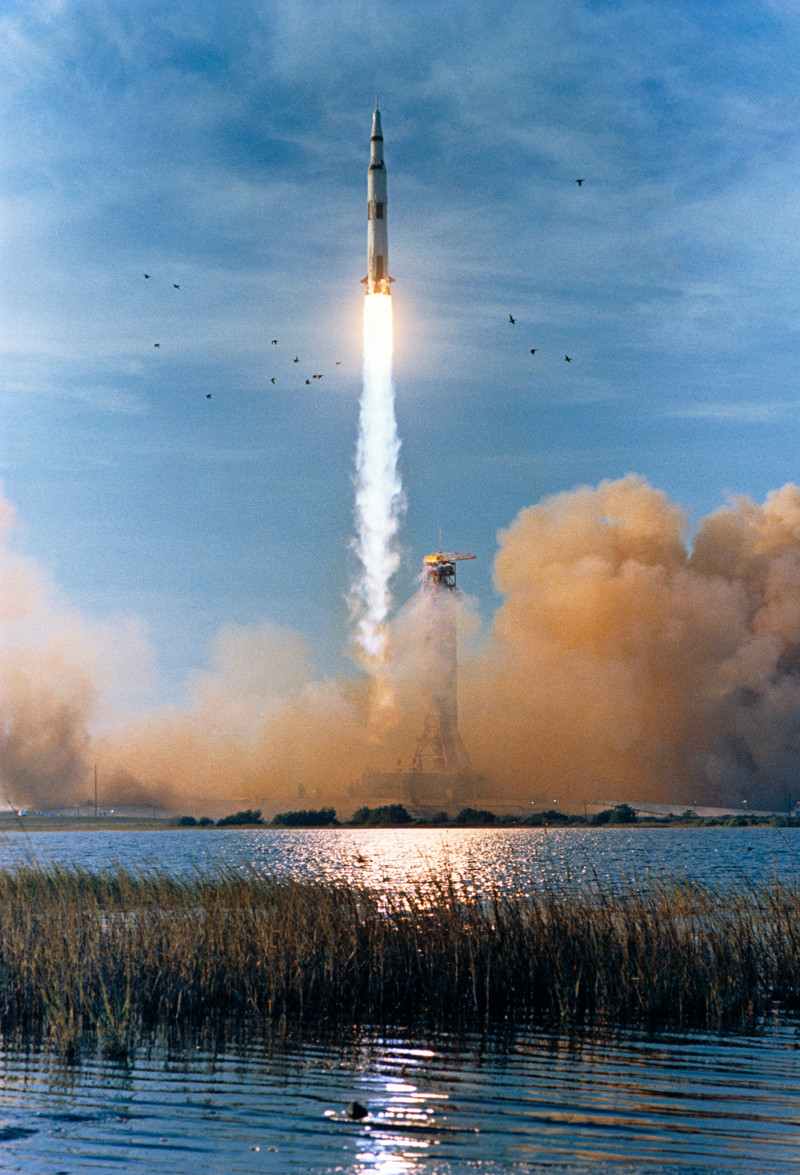
\includegraphics[width=0.9\textwidth]{apollo8-highres.jpg}
\ECC

}

\frame{\frametitle{\bf The dream of flight}

\large

People have dreamed of flying for ages, in all countries and since the earliest days of history.

\BS

\BCC
\column{0.5\textwidth}
\BC
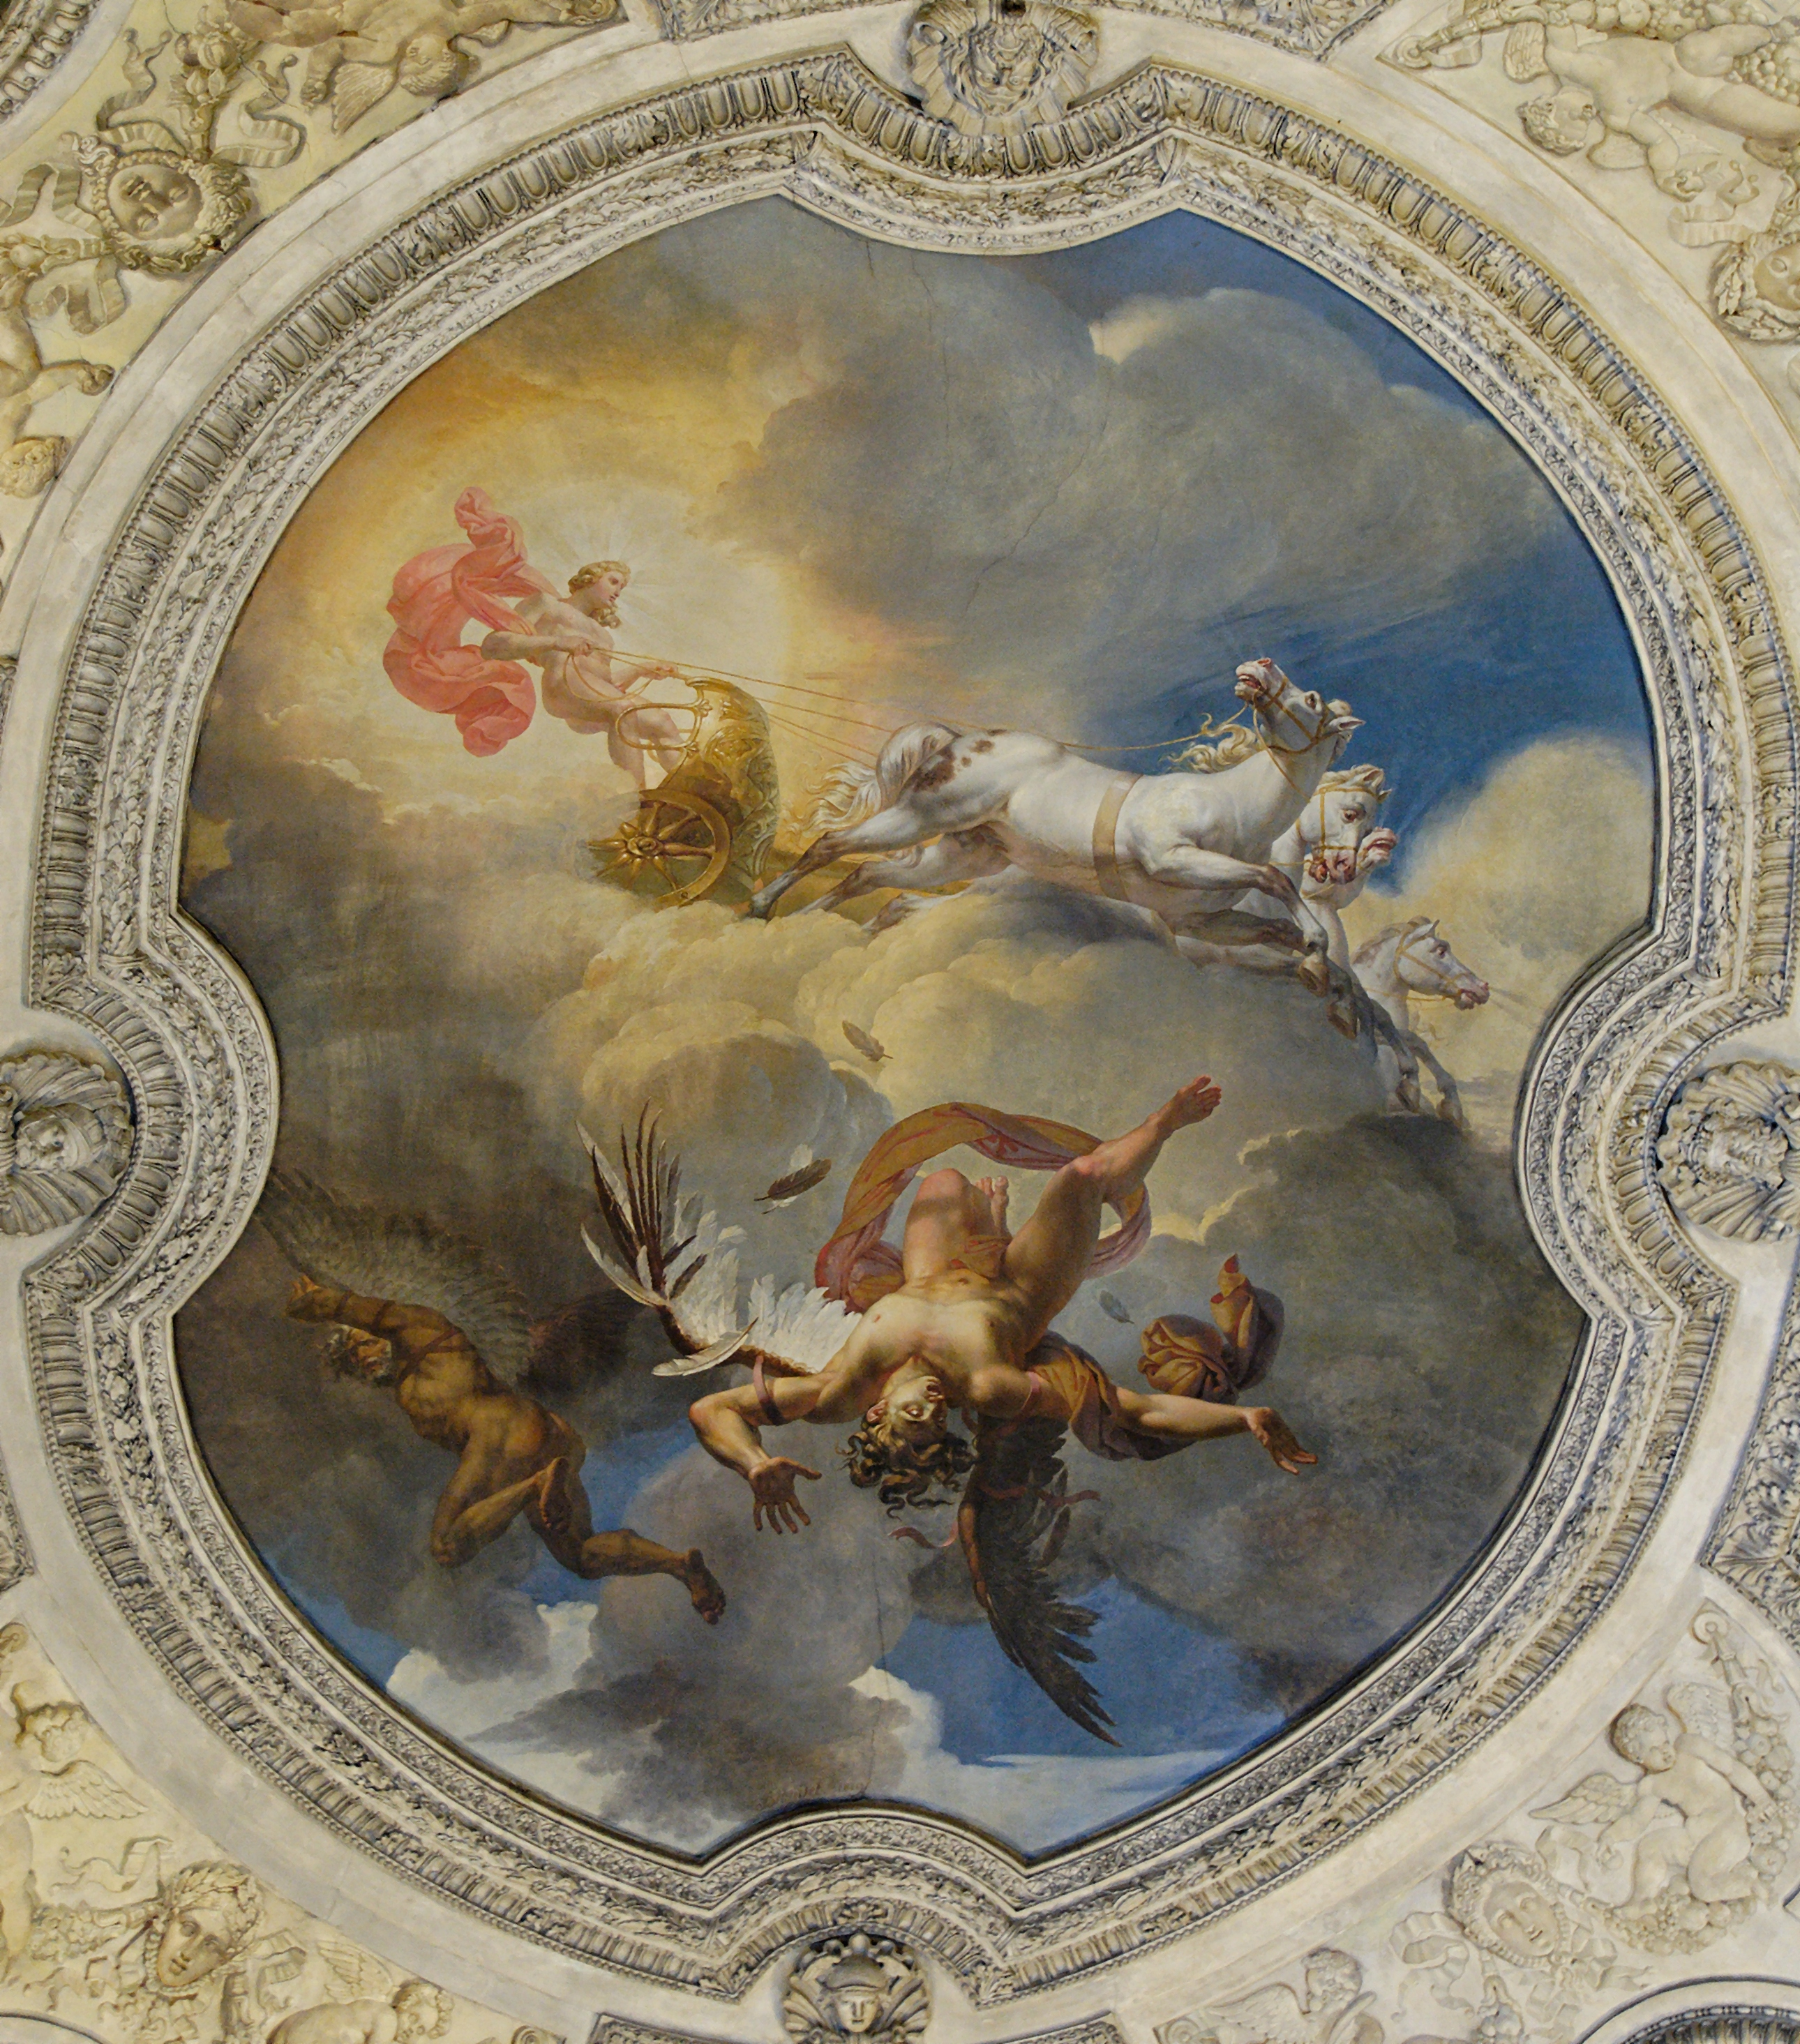
\includegraphics[width=0.95\textwidth]{fall-of-icarus.jpg}
\EC
\column{0.5\textwidth}
\BI
\item Often our dream of flight was a symbol of hubris: ``mortals should know their place''
\item Icarus and Daedalus...
\EI
\ECC
}

\frame{\frametitle{\bf The dream of flight}

\large

People have dreamed of flying for ages, in all countries and since the earliest days of history.

\BS

\BCC
\column{0.5\textwidth}
\normalsize
Leonardo da Vinci (Italian, 1452-1519):
\BI
\item Embodied the humanist spirit of the Renaissance: ``yes, we {\it can}!''
\item Skilled at science, philosophy, engineering, and art
\item ... and used them all to enhance each other
\item Like so many others, dreamed of flying...
\item Was a Ninja Turtle, or my childhood was a lie
\EI

\column{0.5\textwidth}
\BC
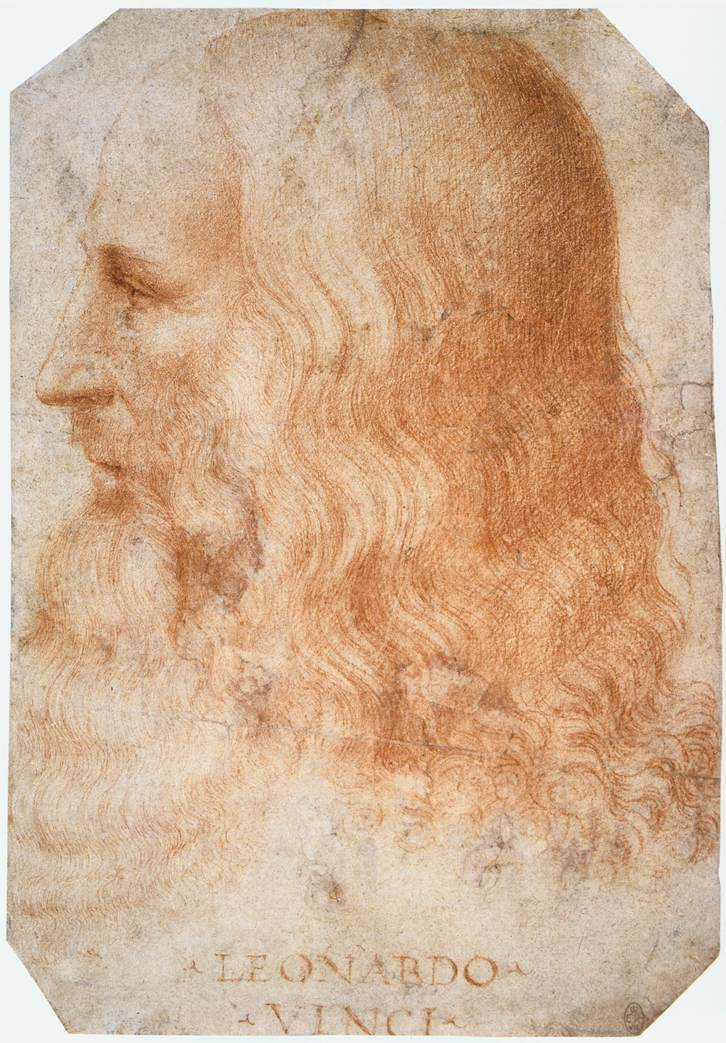
\includegraphics[width=0.7\textwidth]{da-vinci.jpg}
\EC
\ECC
}


\frame{\frametitle{\bf The ``Renaissance man'' (and woman!)}
\large

The Renaissance admired versatility; the ``Renaissance man'' was someone whose skill wasn't confined to one field.

\BS

\BC
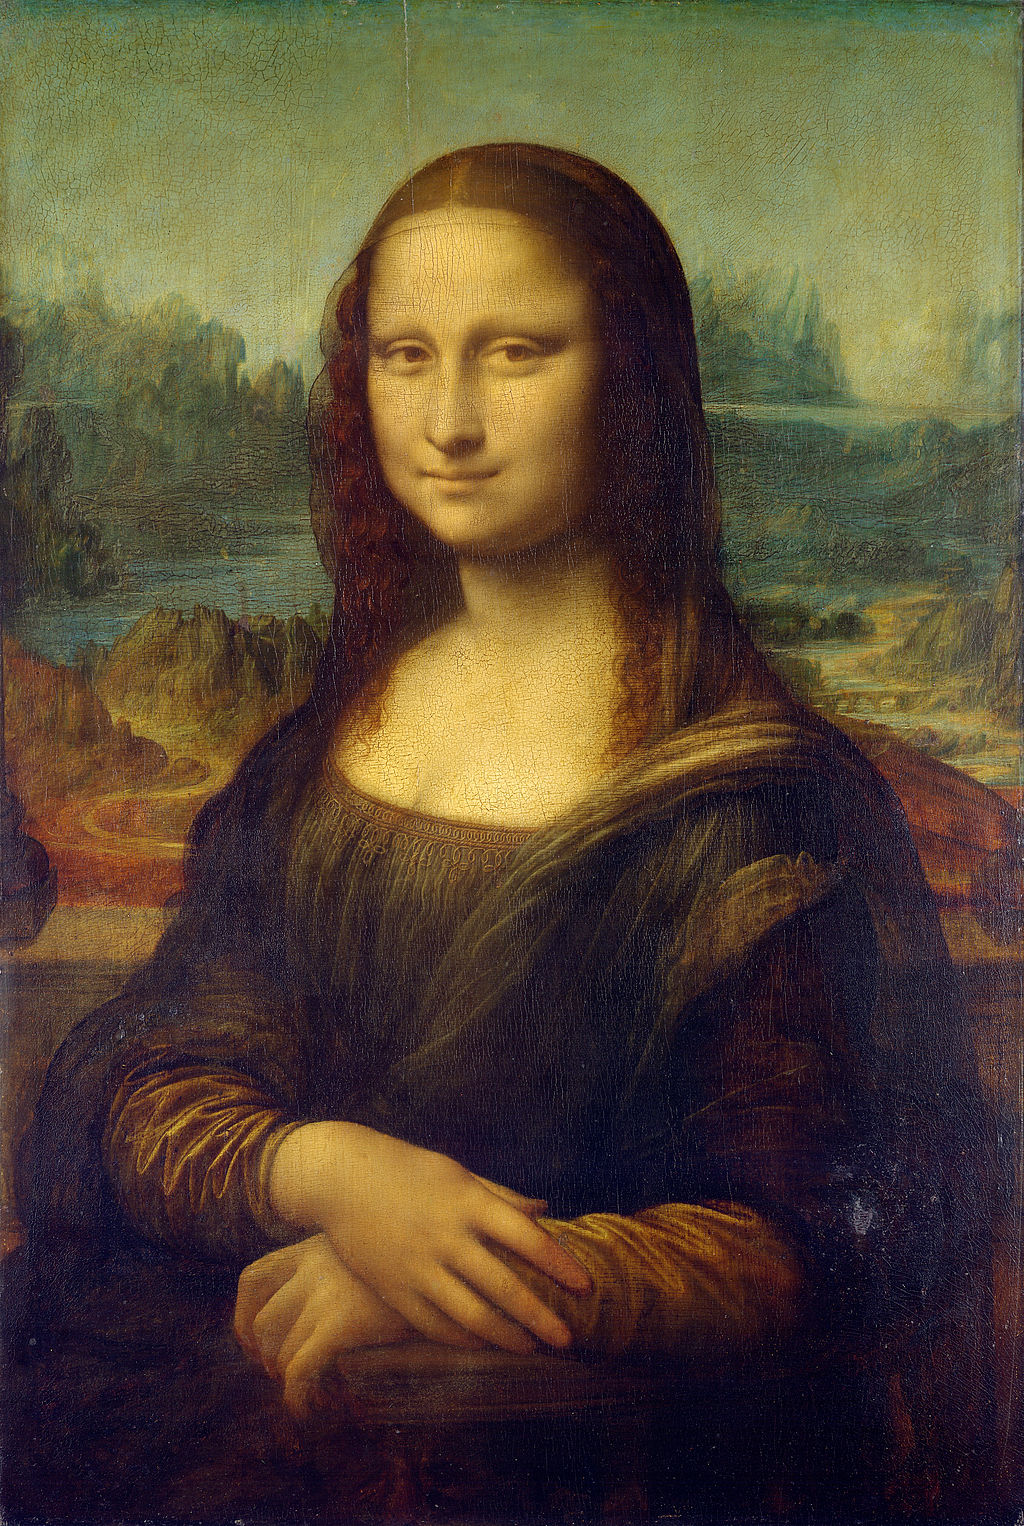
\includegraphics[height=0.5\textwidth]{mona-lisa.jpg}
\hspace{1in}
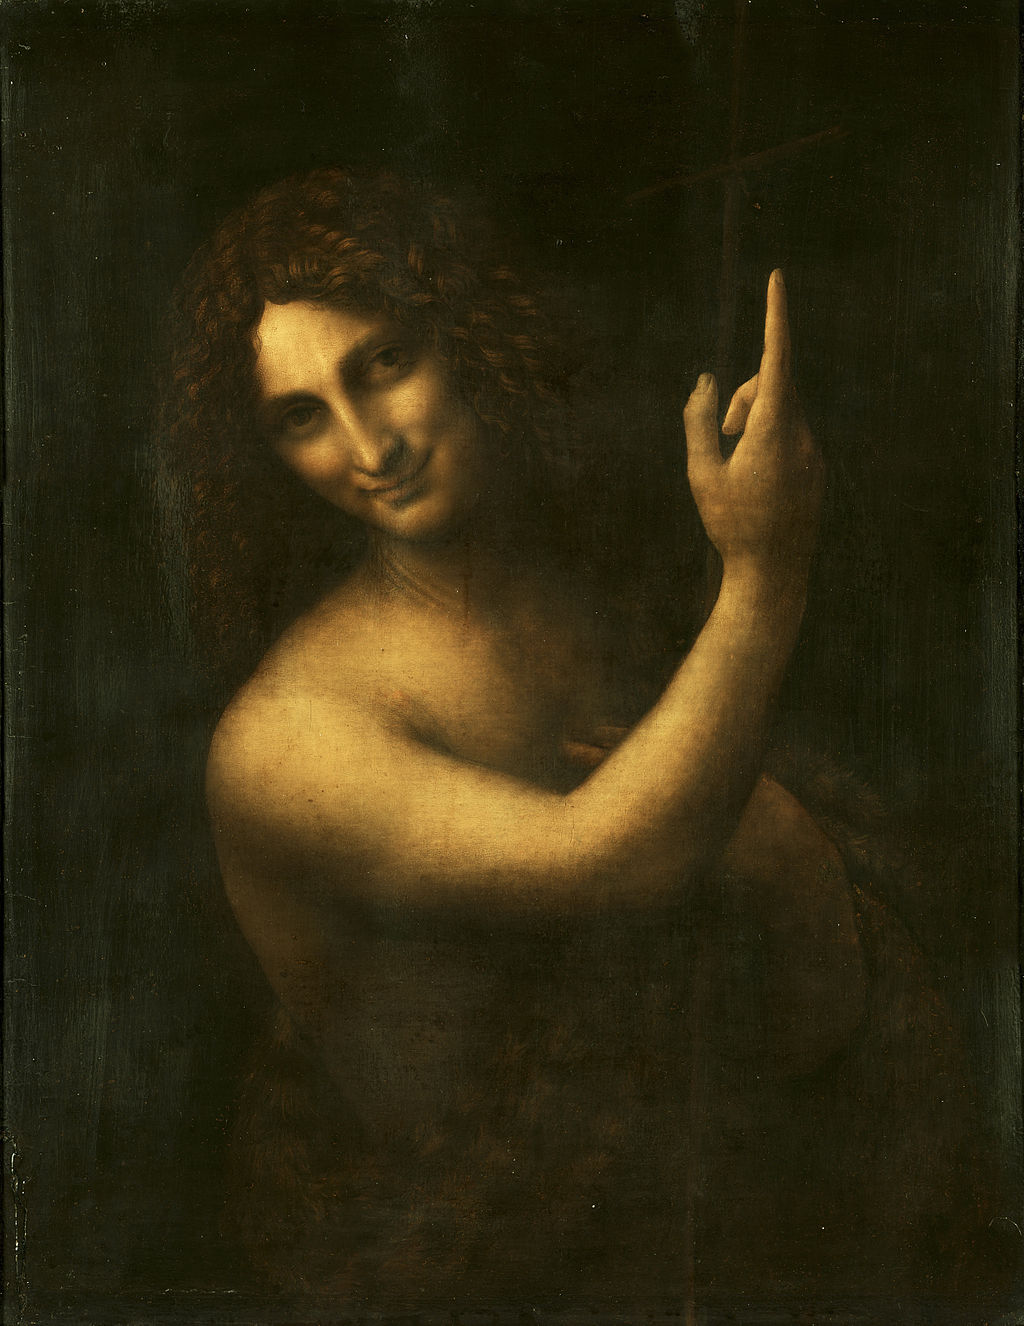
\includegraphics[height=0.5\textwidth]{john-the-baptist.jpg}
\EC
}

\frame{\frametitle{\bf The ``Renaissance man'' (and woman!)}
\large

The Renaissance admired versatility; the ``Renaissance man'' was someone whose skill wasn't confined to one field.

\BS

\BC
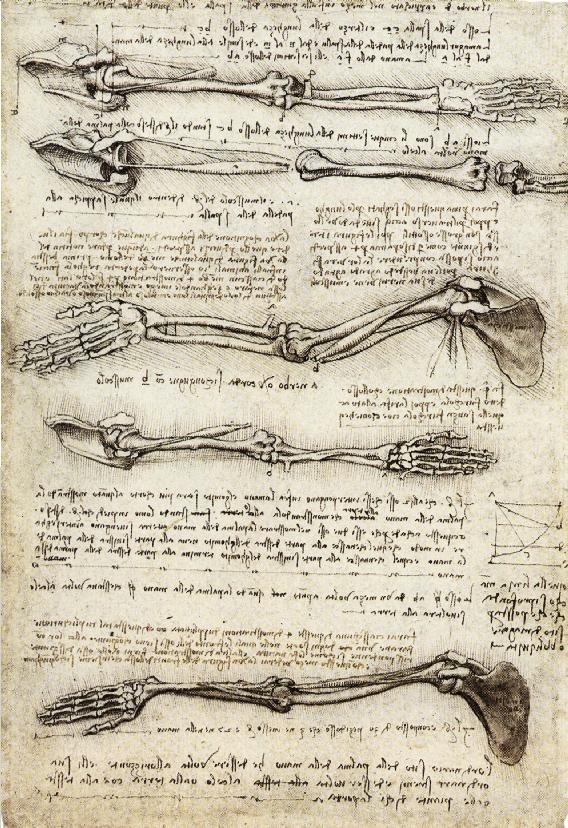
\includegraphics[height=0.5\textwidth]{da-vinci-arm.jpg}
\hspace{1in}
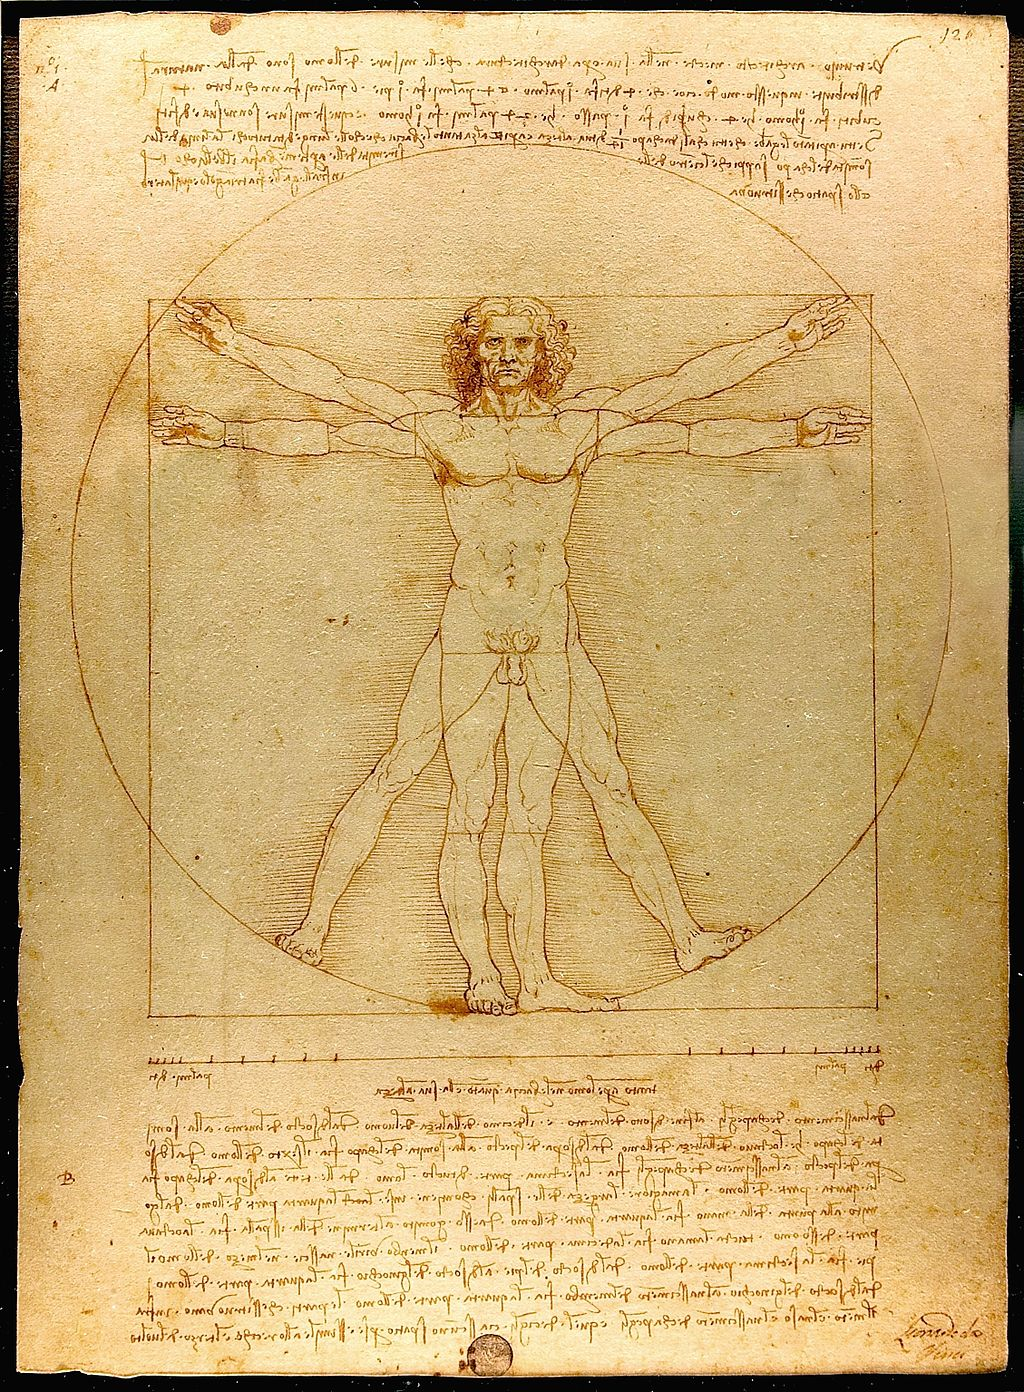
\includegraphics[height=0.5\textwidth]{vitruvian-man.jpg}
\EC
}

\frame{\frametitle{\bf Science as a liberal art}
\large

There's a reason this class is in the ``College of Arts and Sciences''.

\BS

Understanding the world around us was once ``natural philosophy'' -- another branch of the unified whole of learning.

\BS

Some of you may go on to become doctors -- not of physics or literature or engineering, but {\it philosophy}.

\BS

``Science'' just means knowledge: \it Suos cultores scientia coronat...\rm

\BS

It's not ``science and the liberal arts'' -- science {\it is} a liberal art.

\BS

\pause

When you can, be like da Vinci...
}

\frame{\frametitle{\bf da Vinci and flight}
\large

da Vinci dreamed of flying, and wrote a treatise on birds -- and made diagrams for flying machines.

\BS

\BBC
\HC
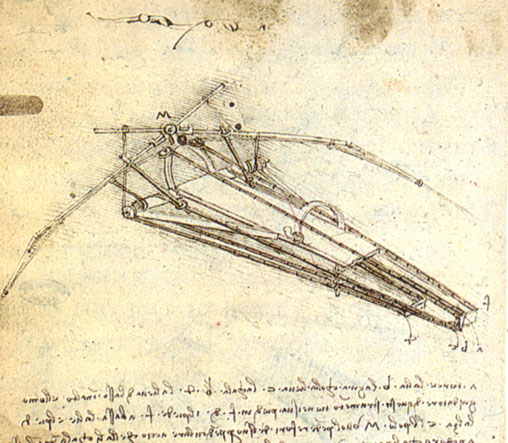
\includegraphics[width=\textwidth]{da-vinci-flying-machine.jpg}
\HC
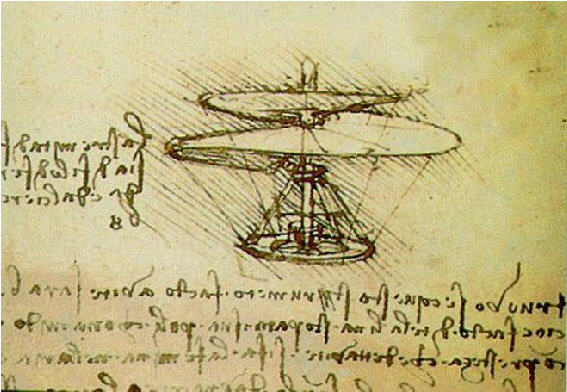
\includegraphics[width=\textwidth]{da-vinci-helicopter.jpg}
\EEC
\BS

Unfortunately, people don't just lack wings -- they lack enough {\color{Red}power}.

\BS

(Human: 60 kg, 400 watts; duck, 1 kg, 100+ watts)

\BS

That's 14 times more power per gram for the duck!
}

\frame{\frametitle{\bf Power + wings = flight!}

Push yourself forward, use wings to push downward on the air (flapping or not), and you can fly!

\BS\pause

Well, not quite -- you have to figure out how to {\it steer}, which is the hard part. (You push on the air...)

\BS\pause

In 1903 Wilbur and Orville Wright put an internal combustion engine on a winged machine, put a propeller on the front, added devices to steer, and invented the airplane.

\BS
\BC
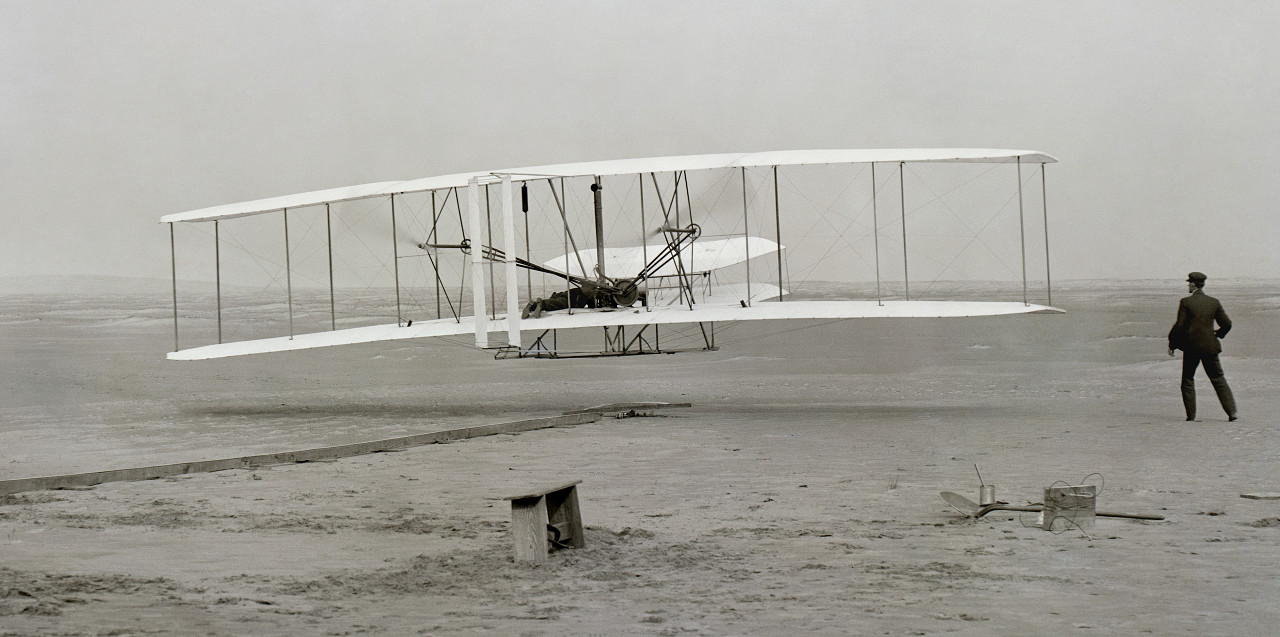
\includegraphics[width=0.7\textwidth]{wright-brothers-flight.jpg}
\EC
}

\frame{\frametitle{\bf The dream of flight, in the waking world...}

\large

\BCC
\HC
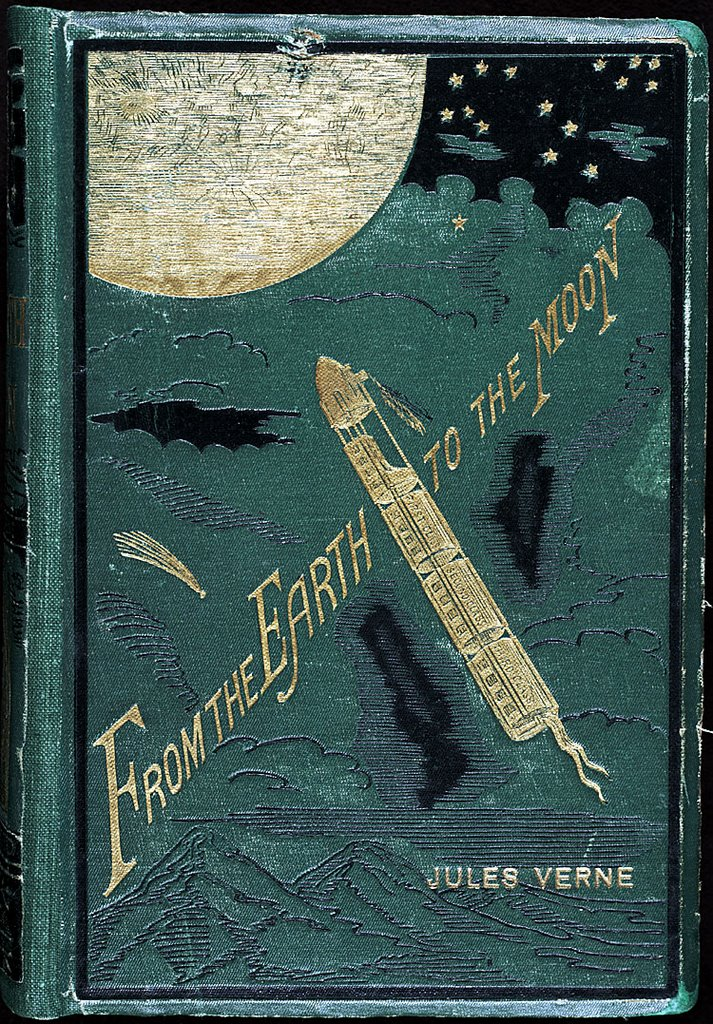
\includegraphics[width=0.8\textwidth]{earth-to-moon.jpg}
\HC
We can fly! Even before that, people were dreaming of going to the Moon and beyond.

\BS
\BI
\small
\item 1865: Verne wrote a book in which Baltimoreans shoot themselves to the Moon in a giant cannon
\item Verne did the math for the size of the gun required and got it right
\item It would have worked!
\item ... the acceleration would have squashed the people, though...
\EI
\ECC
}

\frame{
\Large
A giant cannon won't work. Can we use Wilber and Orville's airplane to go to the Moon?

\BS\BS
\color{A}A: Yep! \\\BS
\color{B}B: Nope; it won't work at all \\\BS
\color{C}C: Sort of -- you can propel yourself, but you can't steer \\\BS
}


\frame{\frametitle{\bf Newton's third law}
\large
Remember gravity?

$$
F = \frac{Gm_1m_2}{r^2}
$$

\normalsize

{\color{Red}``The Sun's pull on the Earth is the same as the Earth's pull on the Sun''}

\BS\pause

This is a general principle of physics:

\BS

{\color{Red}``If A pushes forwards on B, then B must push backwards on A.''}

\BS

How does a propeller work? ``The airplane pushes backwards on the air; the air pushes forwards on the airplane''.

\pause

``A spaceplane pushes backwards on the ... drat, there's no air in space.''

\pause\BS\BS

\BC

\scriptsize (Forget that ``action/reaction'' stuff -- ``action'' meant something specific to Newton that it doesn't mean today.)
\EC
}


\frame{\frametitle{\bf Rockets}

Simple solution, first used in East Asia: carry gas (or anything else) with you, and push it out the back!

\BS

\BCC
\HC

The Chinese had been using rockets in warfare as early as 1280, using the gunpowder also developed in China.

\BS

The Koreans and Mongolians quickly adopted the new weapon, and the technology spread around Eurasia in the next few centuries.

\HC
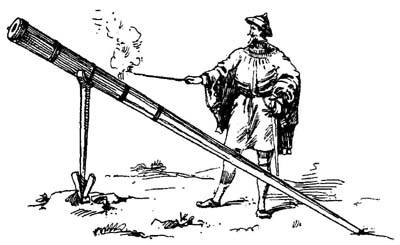
\includegraphics[width=\textwidth]{chinese-rocket.jpg}
\ECC

\BS

This works in space: ``I push backwards on the gas I've brought with me; it pushes forwards on me''
}

\frame{\frametitle{\bf Tsiolkovsky: making rockets precise}

The Russian scientist Konstantin Tsiolkovsky (1857-1935) was the first to study the physics of rocketry in depth. (He also studied music
and the problem of poverty.)

\BS

He discovered the {\it rocket equation}, which describes the performance of a perfect, ideal rocket:

$$
\Delta V = v_e \ln F
$$

Here:

\BI
\item $\Delta V$ is the speed that the rocket will be traveling after it burns its fuel
\BI
\item To escape Earth's gravity: about 11 kilometers/second (calculated by Tsiolkovsky)
\EI
\item $v_e$ is the exhaust velocity of the rocket (how fast the gas comes out the back)
\item $F$ is how many times bigger the rocket is than its payload
\BI
\item Here ``payload'' means every part of the rocket that isn't fuel
\EI
\EI

We can make the math easier and rearrange this:

$$
F = (2.719)^{V/v_e}
$$

or

$$
F = 10^{0.43 \frac{V}{v_e}}
$$
}

\frame{\frametitle{\bf Tsiolkovsky: making rockets precise}

Tsiolkovsky realized that rockets could take us to space, and wrote about this in 1903: ``Exploration of Cosmic Space by Means of Rocket Devices''

\BS


But what kind of fuel is needed? Let's make a table here. Suppose we want to lift a ton to orbit; how much fuel do we need?

\BS

\normalsize
% Please add the following required packages to your document preamble:
\BC% \usepackage{booktabs}
\begin{tabular}{@{}ll@{}}
\toprule
Fuel exhaust speed            & Fuel needed              \\ \midrule
1000 km/hr                    & 300 million billion tons \\
2000 km/hr                    & 5.5 million tons         \\
3000 km/hr                    & 680,000 tons             \\
5000 km/hr                    & 3100 tons                \\
9000 km/hr (solid rockets)    & 87 tons                  \\
15400 km/hr (hydrogen/oxygen) & 13 tons                  \\
104000 km/hr (ion thrusters)  & 470 kilograms      \\
\toprule
\end{tabular}
\EC

The problem with rockets: you have to carry your fuel with you. The less efficient your fuel is, the more fuel you need, so you need more fuel to carry
that fuel...

\BS

And, if you want to come back from wherever you went, you need even {\it more} fuel...
}


\frame{\frametitle{\bf Robert Goddard: making rockets}

\large

Robert Goddard (American; 1882-1945) had a long-running interest in rocketry as a means to get to space. He:

\BI
\item took Tsiolkovsky's ideas and put them into practice
\item realized that a specially-shaped rocket nozzle could greatly increase exhaust speeds (remember how much this matters!)
\item achieved exhaust speeds of 8600 km/hr
\pause
\item believed that a rocket could reach the Moon!
\EI

For the first time, we have a plan: a machine whose workings we understand that can get us to the Moon! 

\BS
}

\frame{

Not everyone was convinced. 

\it\BS

``[A]fter the rocket quits our air and really starts on its longer journey, its flight would be neither accelerated nor maintained by the explosion of the charges it then might have left. To claim that it would be is to deny a fundamental law of dynamics, and only Dr. Einstein and his chosen dozen, so few and fit, are licensed to do that....
That Professor Goddard, with his ``chair" in Clark College and the countenancing of the Smithsonian Institution, does not know the relation of action and reaction [Newton's third law], and of the need to have something better than a vacuum against which to [push] -- to say that would be absurd. Of course he only seems to lack the knowledge ladled out daily in high schools.''

\BS
\rm
\begin{flushright} --\it The New York Times\rm, 1920\end{flushright}

}

\frame{\frametitle{\bf Rockets as a weapon}

Humanity's dream of flight to the Moon was interrupted by the Second World War, with rockets pressed into service to kill each other.

\BS

All sides in the war used rocket weapons, but the most famous and largest was the German V-2:
\url{https://www.youtube.com/watch?v=94T8VxOOvdI}

\BS

These rockets, designed by a team of German engineers led by Werhner von Braun, were fired across the English Channel at London.
They didn't do much damage, but were terrifying.

\pause\BS

After WWII, the Cold War was on: the Americans and the Soviets thought it was just a matter of time until they were at war. 

\BS

Both sides rushed to capture von Braun and his team; the Americans got there first, and brought them back to Alabama.

\BS

\pause

One of them lived across the street from me when I was a child. Another one was my high school English teacher.

}



\frame{\frametitle{\bf The Cold War}

Both Americans and Soviets lived in constant fear of nuclear war. 

\BS

A rocket that could deliver a nuclear warhead was the ultimate weapon: an ICBM.

\BS

So rocket technology was key to ``winning'' the Cold War.

\BS

Both sides wanted to demonstrate their superiority. The Soviets, however, beat us: showing their mastery of the technology that could be used
to kill tens of millions of Americans in a fraction of an hour.
}

\frame{\frametitle{\bf Sputnik and Vostok}
In 1957, the Soviets got there first, and launched the first satellite: Sputnik. \url{https://www.youtube.com/watch?v=qvPzUAeWZZY}

\pause\BS

This {\it terrified} the Americans: if you can put a satellite in orbit, you can get a thermonuclear bomb anywhere on Earth's surface.
We created NASA in response and desperately tried to catch up, with a concentrated effort to recruit engineers and scientists to work on the project. 

\BS\pause\BS

Then in 1961 the Soviets launched a human to space, Yuri Gagarin, who orbited the Earth and returned safely.

\BC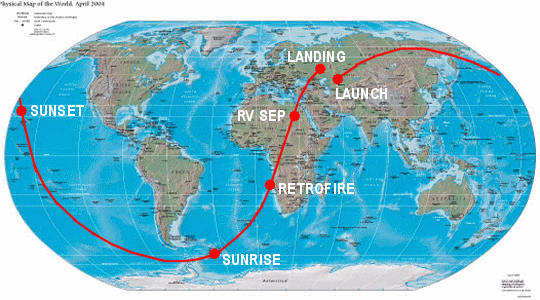
\includegraphics[width=0.6\textwidth]{vostok-1.png}\EC

}

\frame{\frametitle{\bf The American response}
In 1962 the American president John F. Kennedy called for a concentrated, devoted effort to travel to the Moon.

\BS

\url{https://www.youtube.com/watch?v=th5A6ZQ28pE} (excerpts -- full text at \url{http://bit.ly/2gB9L5q})

\pause\BS

The effort took seven years. Before embarking on the mission to build the Moon rocket, we undertook two other flight programs:

\BI
\item Project Mercury: small craft that carried one person, the first American in space Alan Shepard
\item Project Gemini: two-person spacecraft in low-Earth orbit
\BI
\item Life support technology
\item Orbital maneuvering and docking
\item Extravehicular activity (``spacewalks'')
\EI
\EI
}


\frame{\frametitle{\bf The Apollo program}

\BCC
\HC
\BC
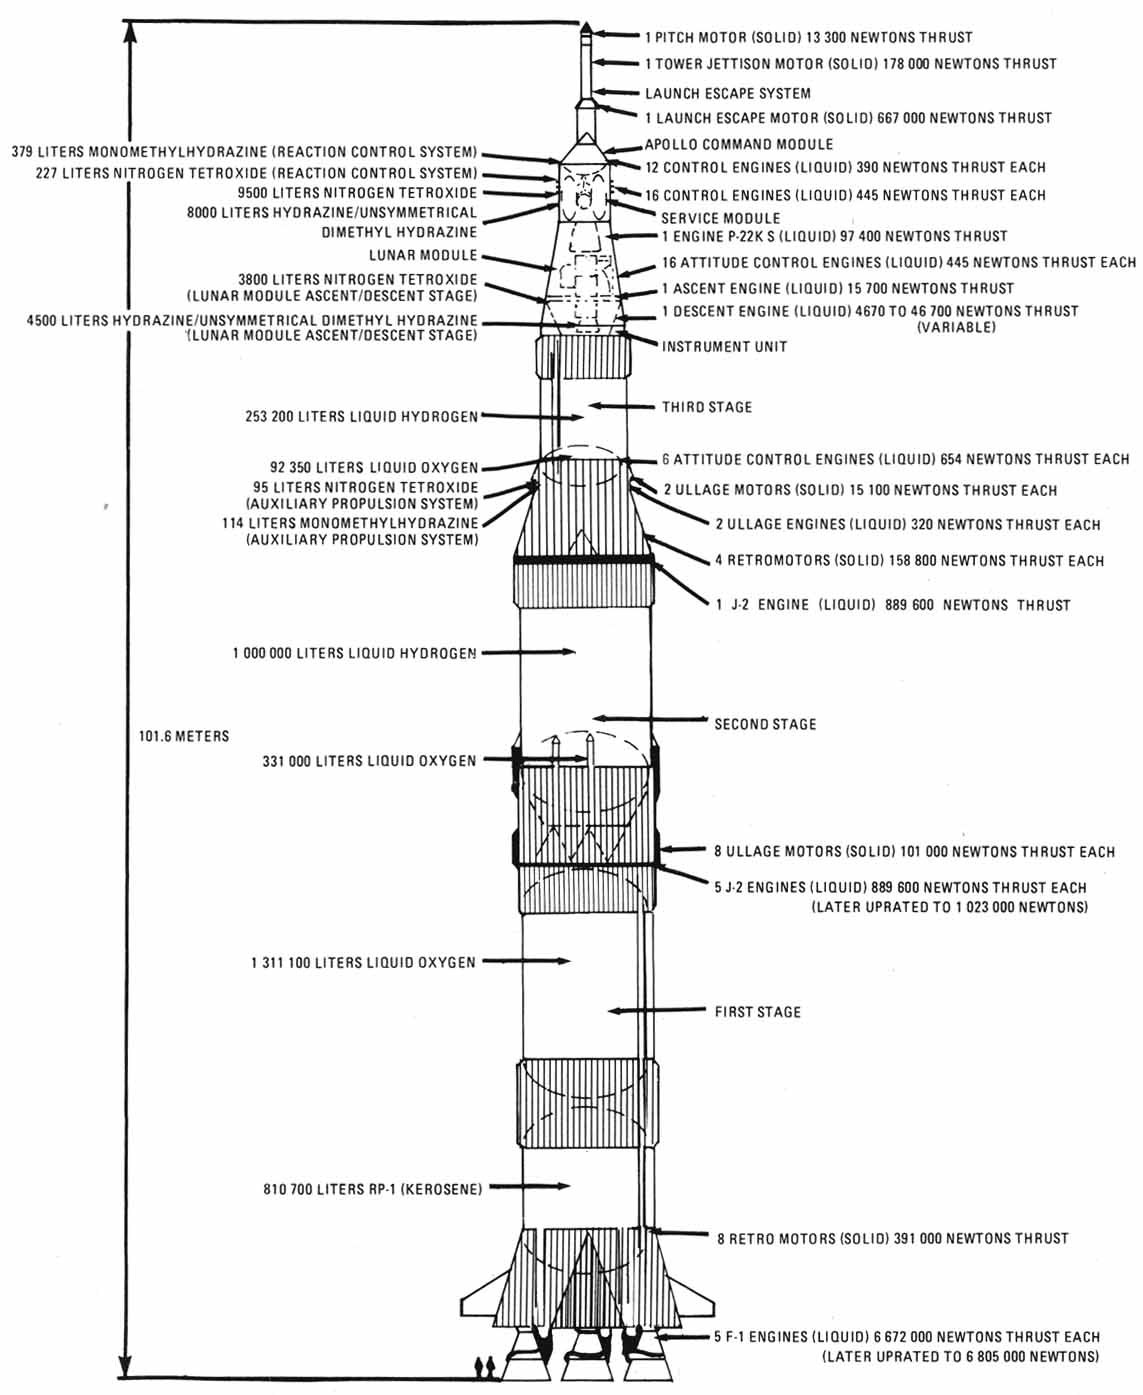
\includegraphics[height=1.1\textwidth]{saturn-v.jpg}
\EC
\HC
NASA set out to build a large rocket, the Saturn V, that could reach the Moon.
\BI
\item Three stages
\item Designed to boost two spacecraft to the Moon
\item ... a command module, designed to stay in lunar orbit
\item ... and a lunar module, designed to land on the Moon itself
\EI
\pause
\url{https://xkcd.com/1133/}
\ECC
}

\frame{\frametitle{\bf The first few flights}
\BCC
\HC
\BI
\item Apollo I (1967): crew chamber pressurized with pure $O_2$
\item Caught fire; all three astronauts died -- Chaffee, White, and Grissom.
\item Seven flights in 1967-1969 tested various pieces of the equipment
\item Apollo 8 and 10 sent astronauts to orbit the Moon itself, but they didn't land
\item Massive engineering challenges required the invention of totally new fields
\pause
\item ``Software engineering'' 
\EI
\HC
\BC
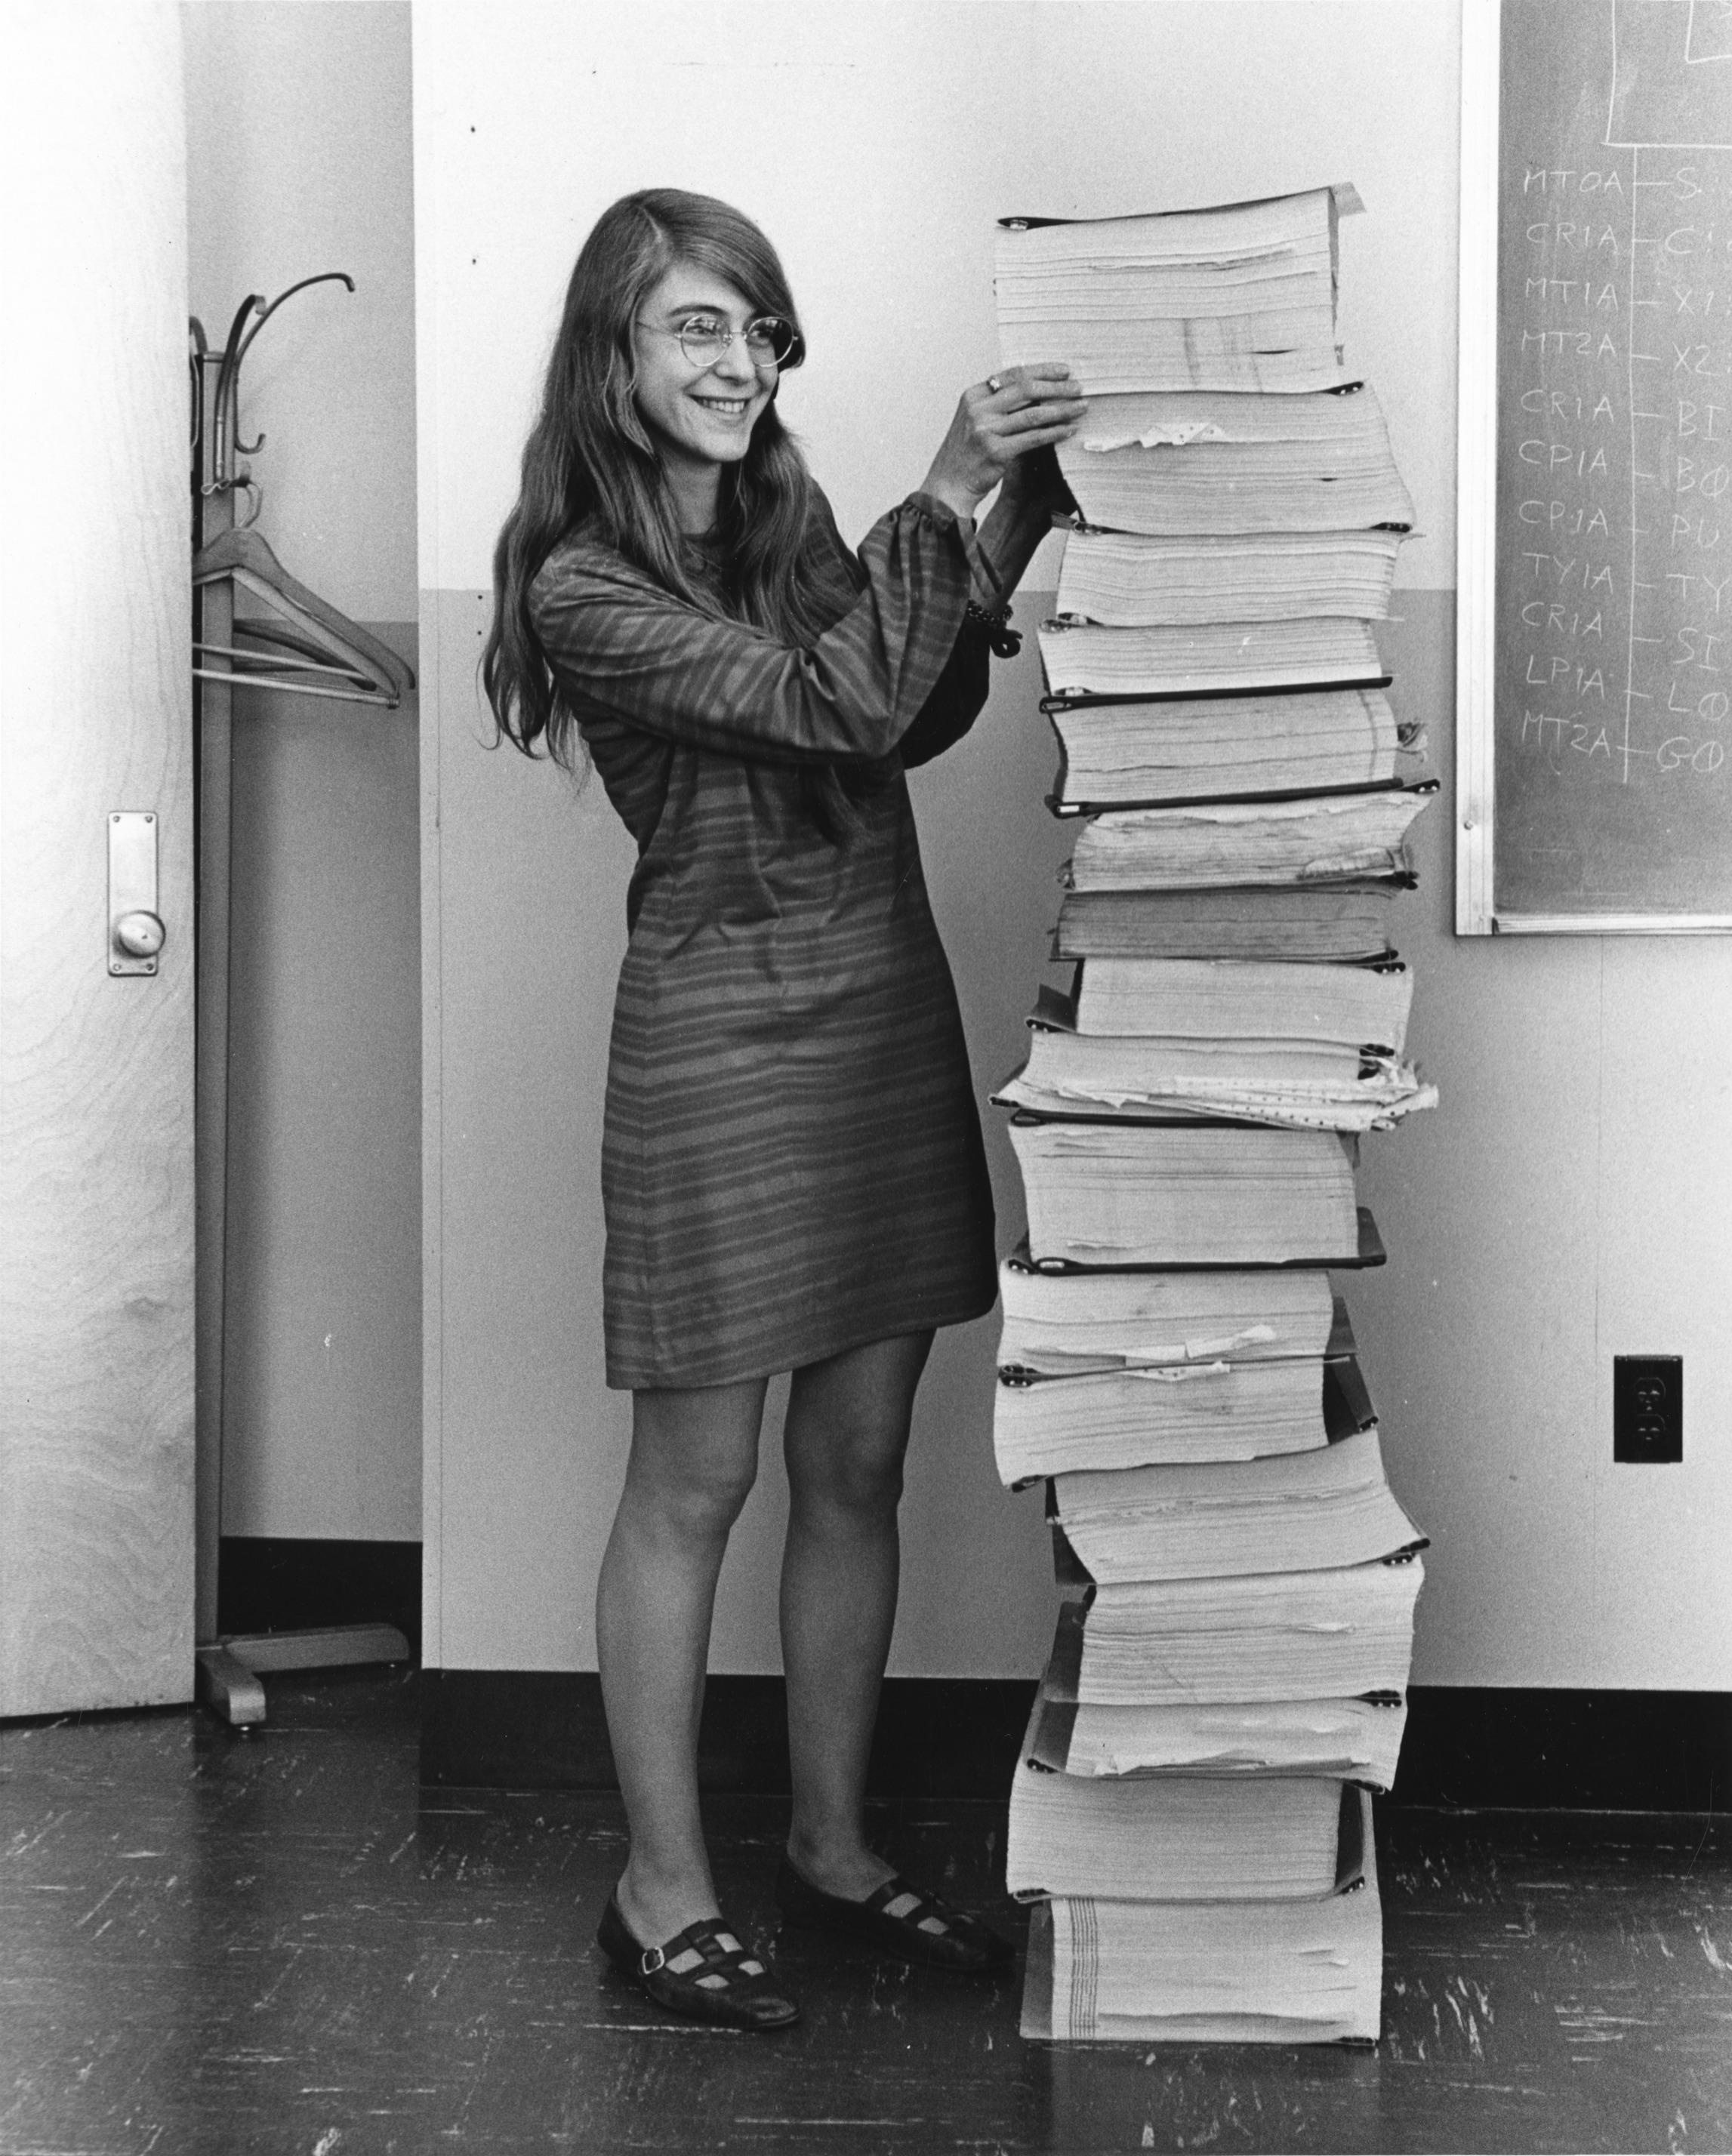
\includegraphics[width=0.9\textwidth]{hamilton.jpg}
\scriptsize

Margaret Hamilton, leader of the MIT team that developed the flight computer software for {\it Apollo}\EC
\ECC
}

\frame{\frametitle{\bf Apollo 11: the Moon, at last!}
Finally, it was time to go for the prize. \url{https://youtu.be/UExTN3\_UOIY}
\pause

\BC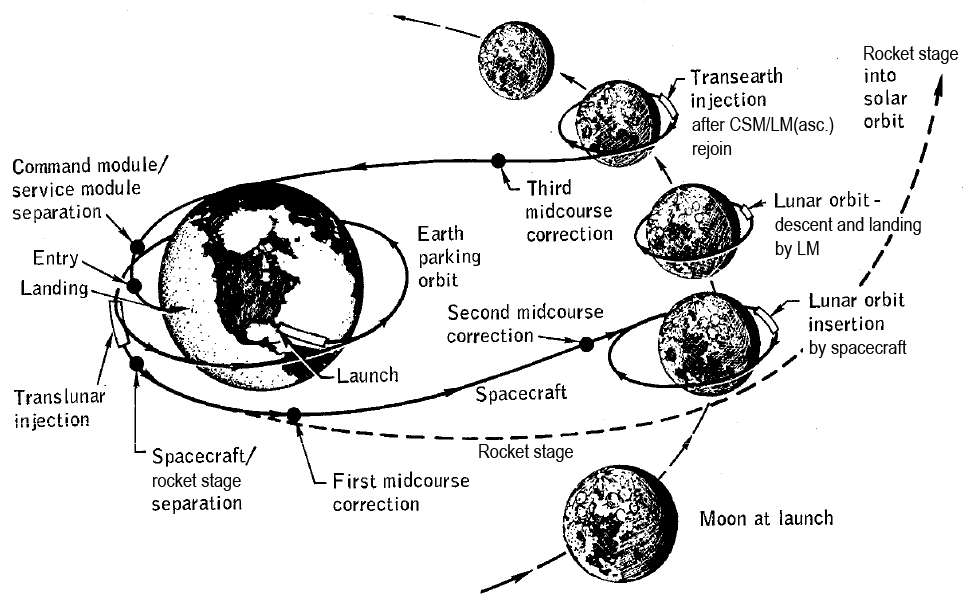
\includegraphics[width=0.8\textwidth]{apollo-program.png}\EC
\url{https://youtu.be/XisDvCTww4M?t=220}
}

\frame{

\it\BS

``[A]fter the rocket quits our air and really starts on its longer journey, its flight would be neither accelerated nor maintained by the explosion of the charges it then might have left. To claim that it would be is to deny a fundamental law of dynamics, and only Dr. Einstein and his chosen dozen, so few and fit, are licensed to do that....
That Professor Goddard, with his ``chair" in Clark College and the countenancing of the Smithsonian Institution, does not know the relation of action and reaction [Newton's third law], and of the need to have something better than a vacuum against which to [push] -- to say that would be absurd. Of course he only seems to lack the knowledge ladled out daily in high schools.''

\BS
\rm
\begin{flushright} --\it The New York Times\rm, 1920\end{flushright}

\pause

``\it Further investigation and experimentation have confirmed the findings of Isaac Newton in the 17th Century and it is now definitely established that a rocket can function in a vacuum as well as in an atmosphere. The \rm Times \it regrets the error.''

\BS
\rm
\begin{flushright} --\it The New York Times\rm, 1969 \end{flushright}
}


\frame{\frametitle{\bf Apollo 11: the Moon, at last!}
On 20 July, 1969, humanity walked on another world for the first time.
\BI
\item Neil Armstrong and Buzz Aldrin descended to the lunar surface
\item Michael Collins stayed in lunar orbit in the Command Module
\item They stayed on the Moon for nearly a day, walking on the surface for two and a half hours
\item They brought back around fifty pounds of moon-rocks
\item Gallery of images: \url{http://www.hq.nasa.gov/alsj/a11/a11\_eva\_thumbs.html}
\EI
}

\frame{\frametitle{\bf The remainder of Apollo}
\BBC
\HC
\BI
\item The USA launched seven more {\it Apollo} missions to the Moon.
\item Six of them made it; one, {\it Apollo 13}, suffered from an explosion en route.
\BI
\item Its story was made into a wonderful film of the same name
\EI
\item 800+ pounds of moon rocks returned to Earth
\item Dozens of hours spent on the lunar surface
\EI
\HC
\BC
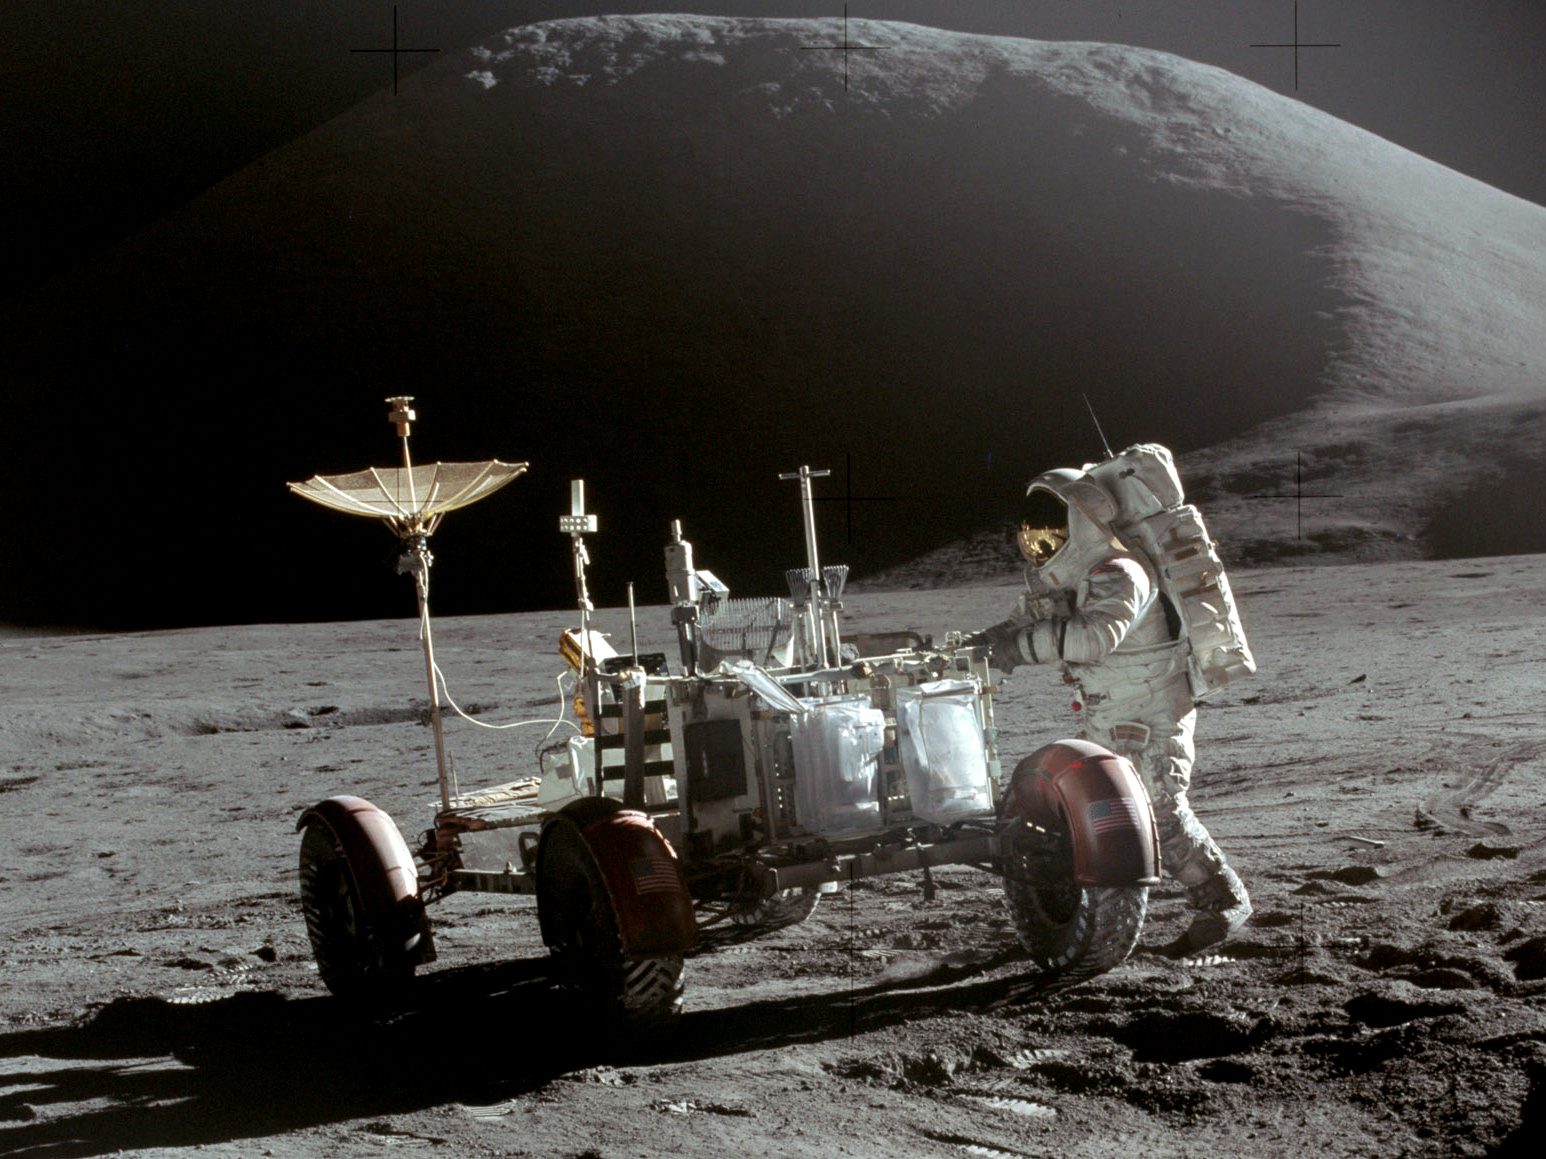
\includegraphics[width=0.9\textwidth]{lunar-rover.jpg}
\EC
\EEC
}

\frame{\BC
\includegraphics[width=0.7\textwidth]{apollo-17.jpg}\EC
}

\frame{\BC
\BBC
\HC
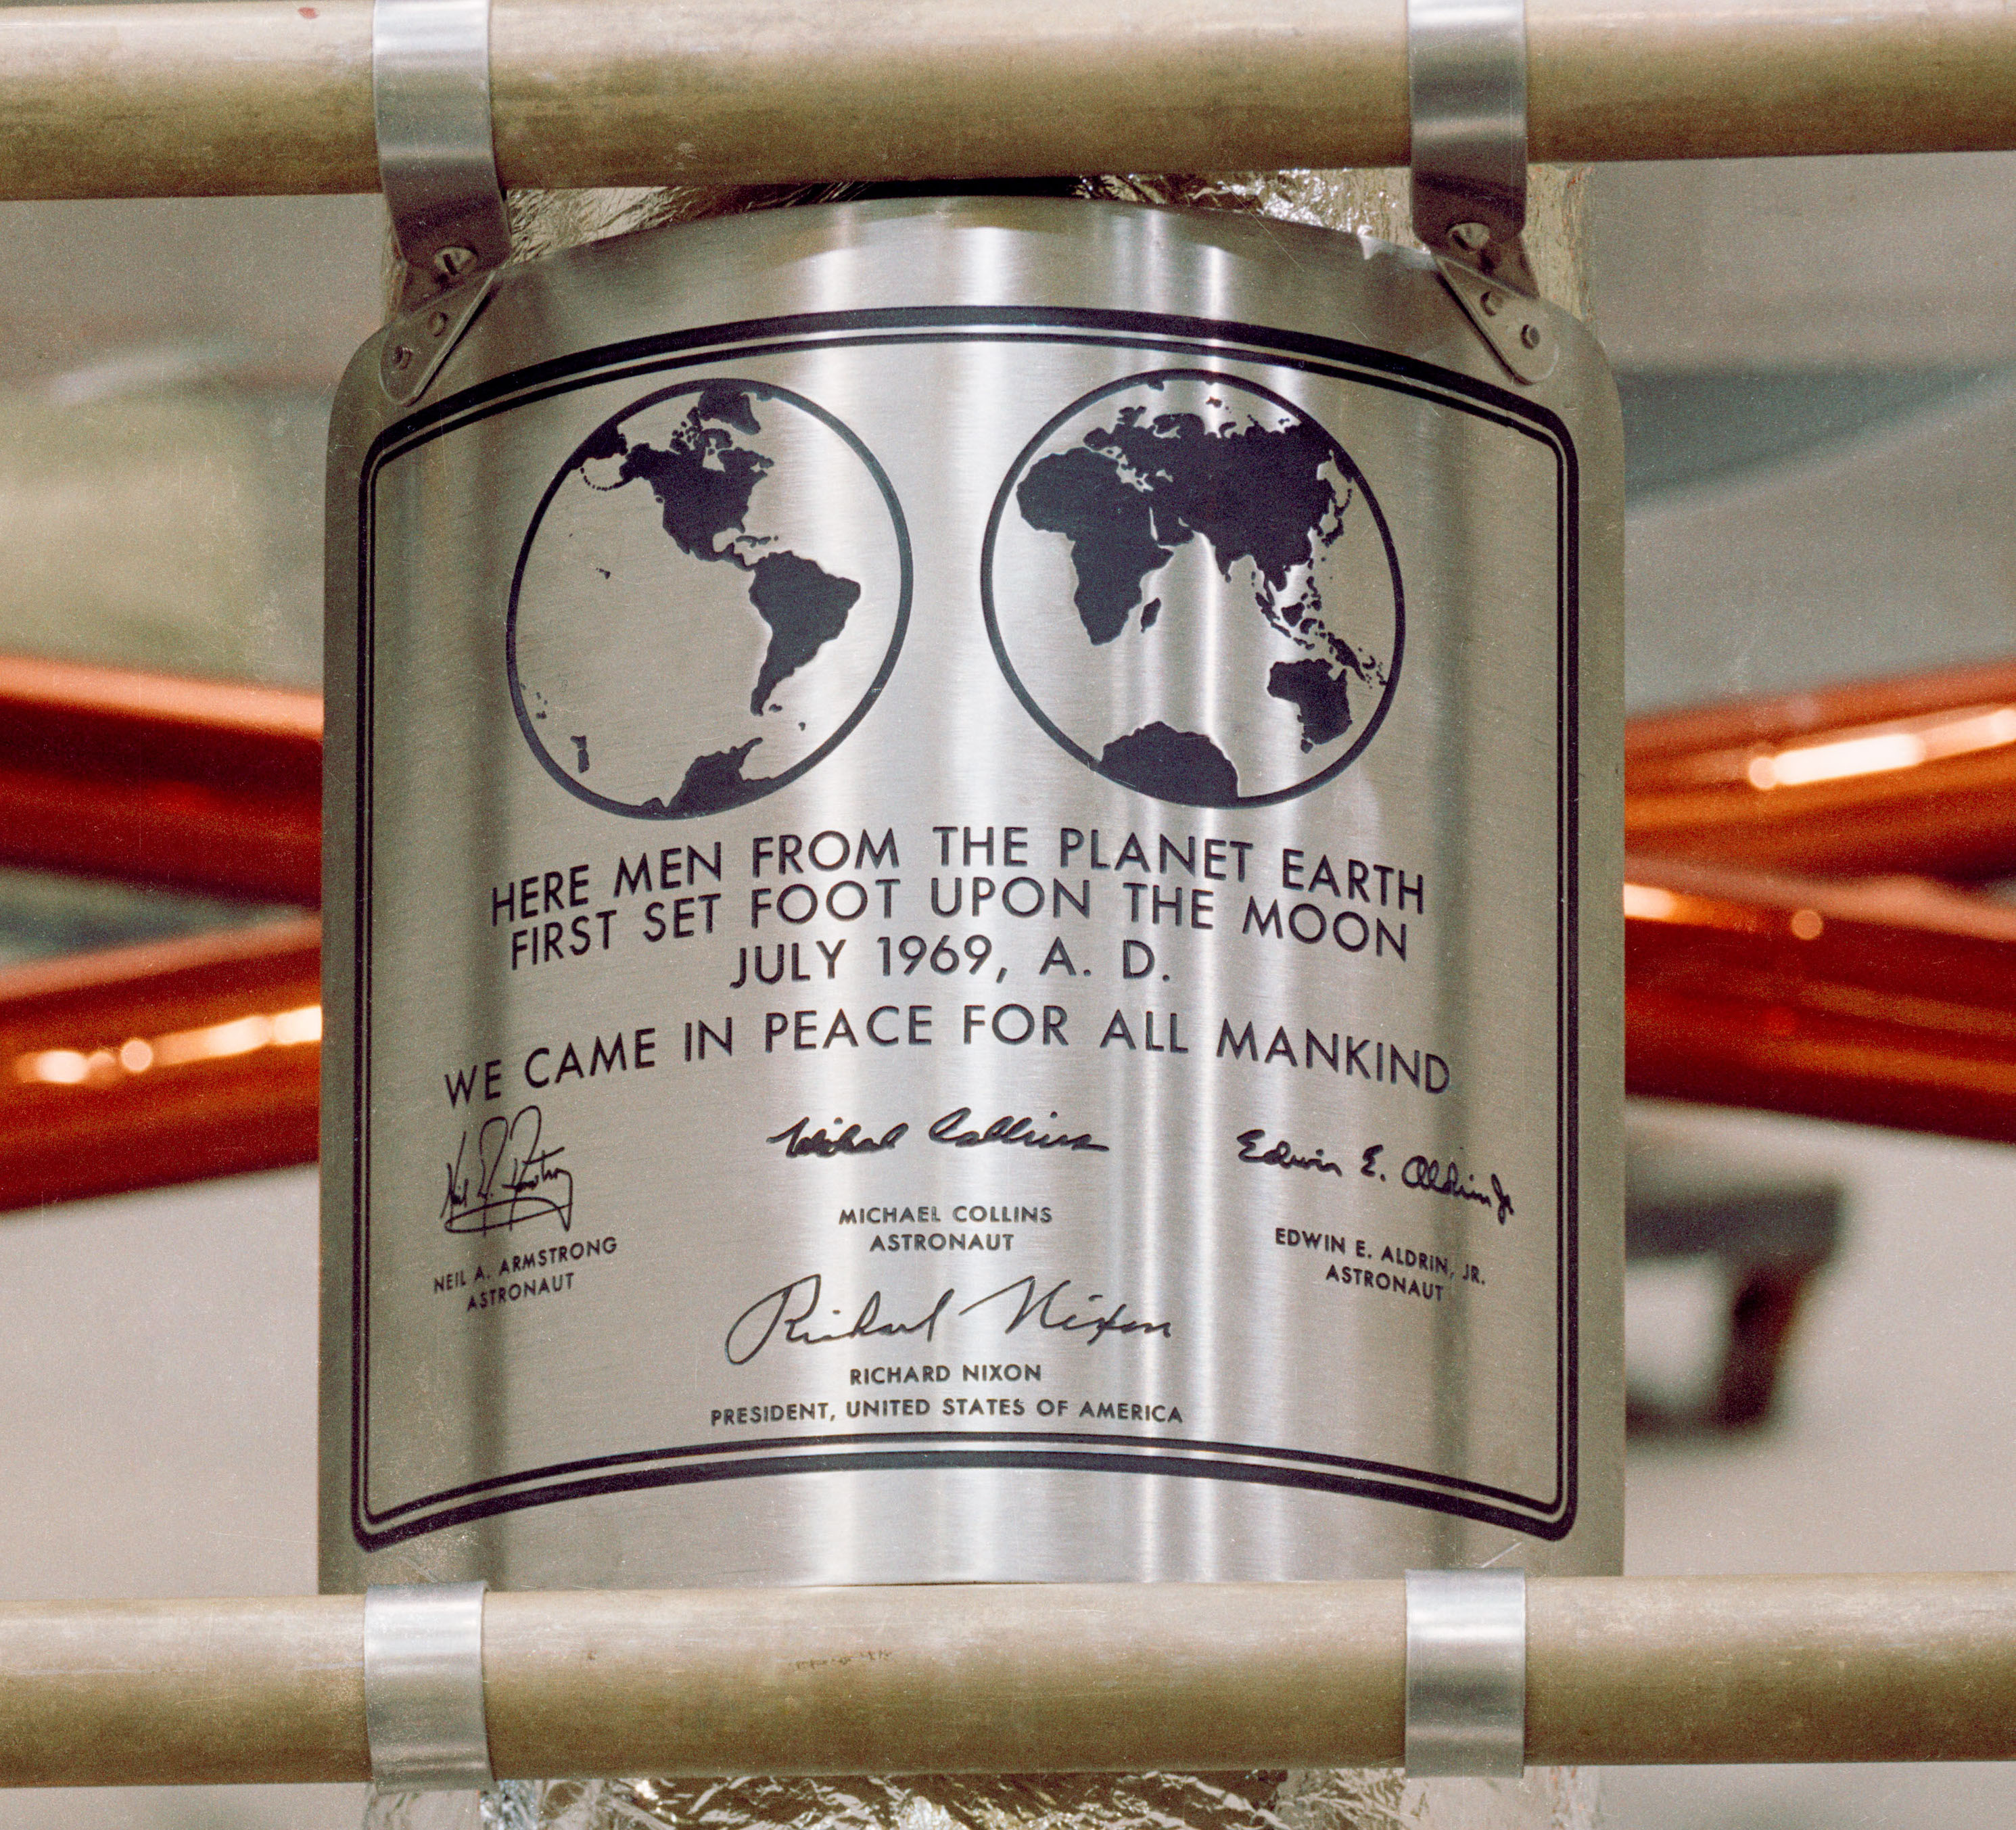
\includegraphics[width=\textwidth]{apollo-11-plaque.jpg}
\HC
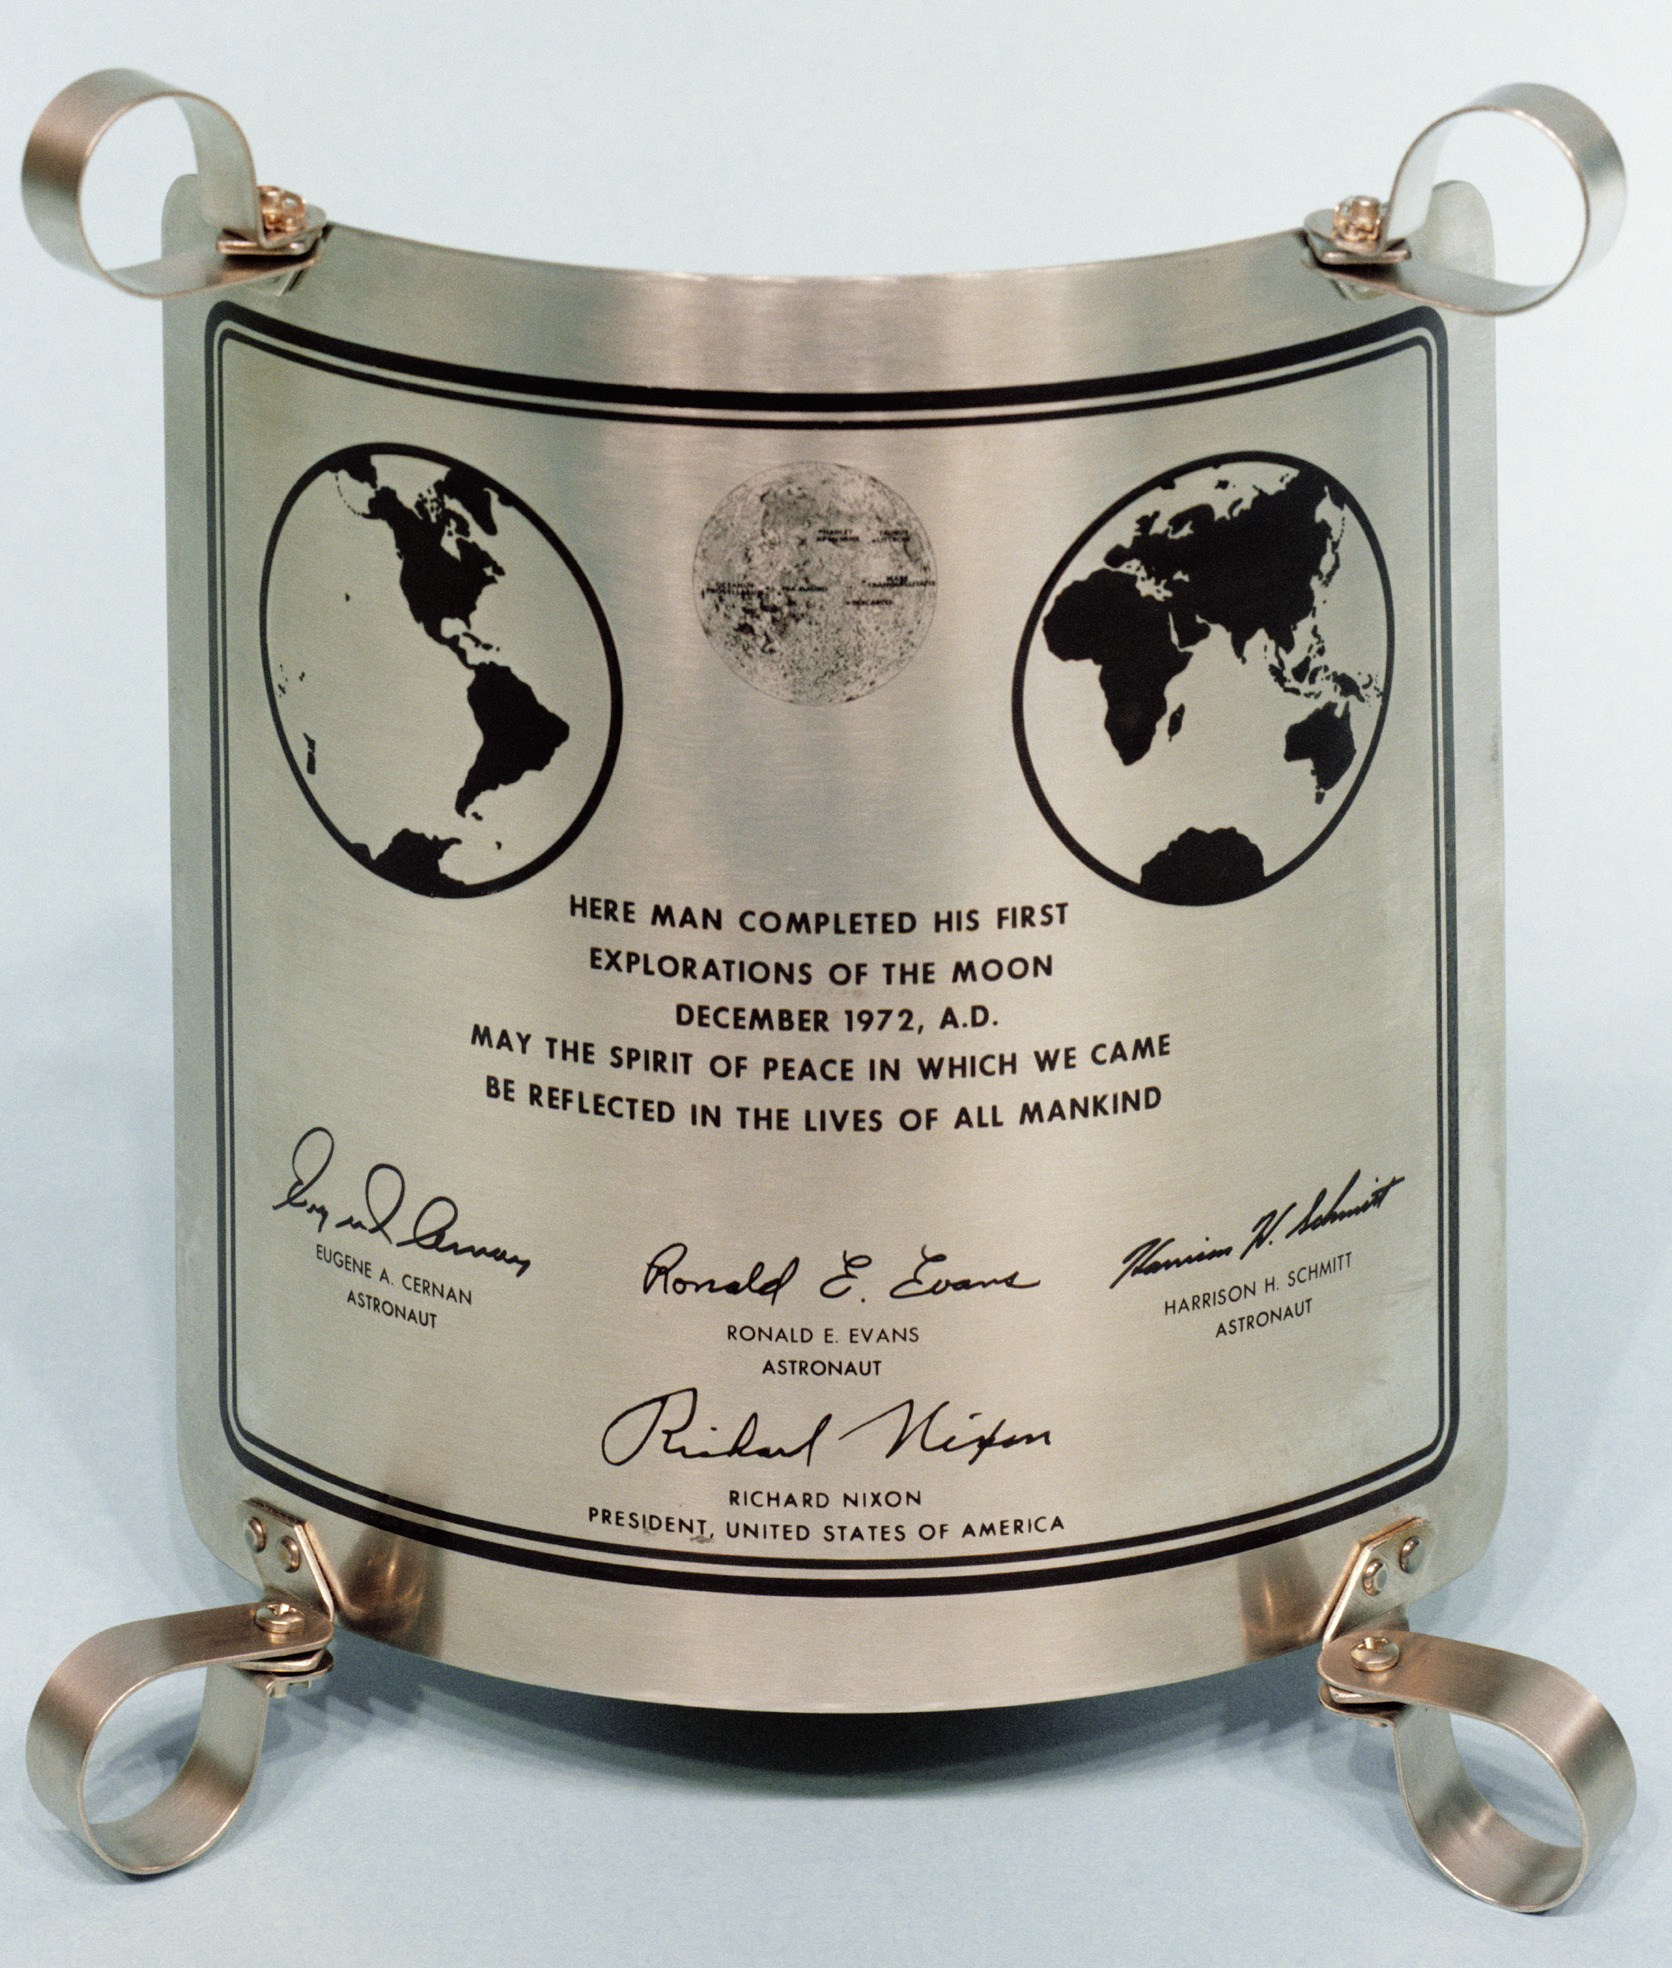
\includegraphics[width=0.9\textwidth]{apollo-17-plaque.jpg}
\EEC
\EC
}


\frame{\frametitle{\bf Forgotten weapons into long-remembered stories...}

\BC
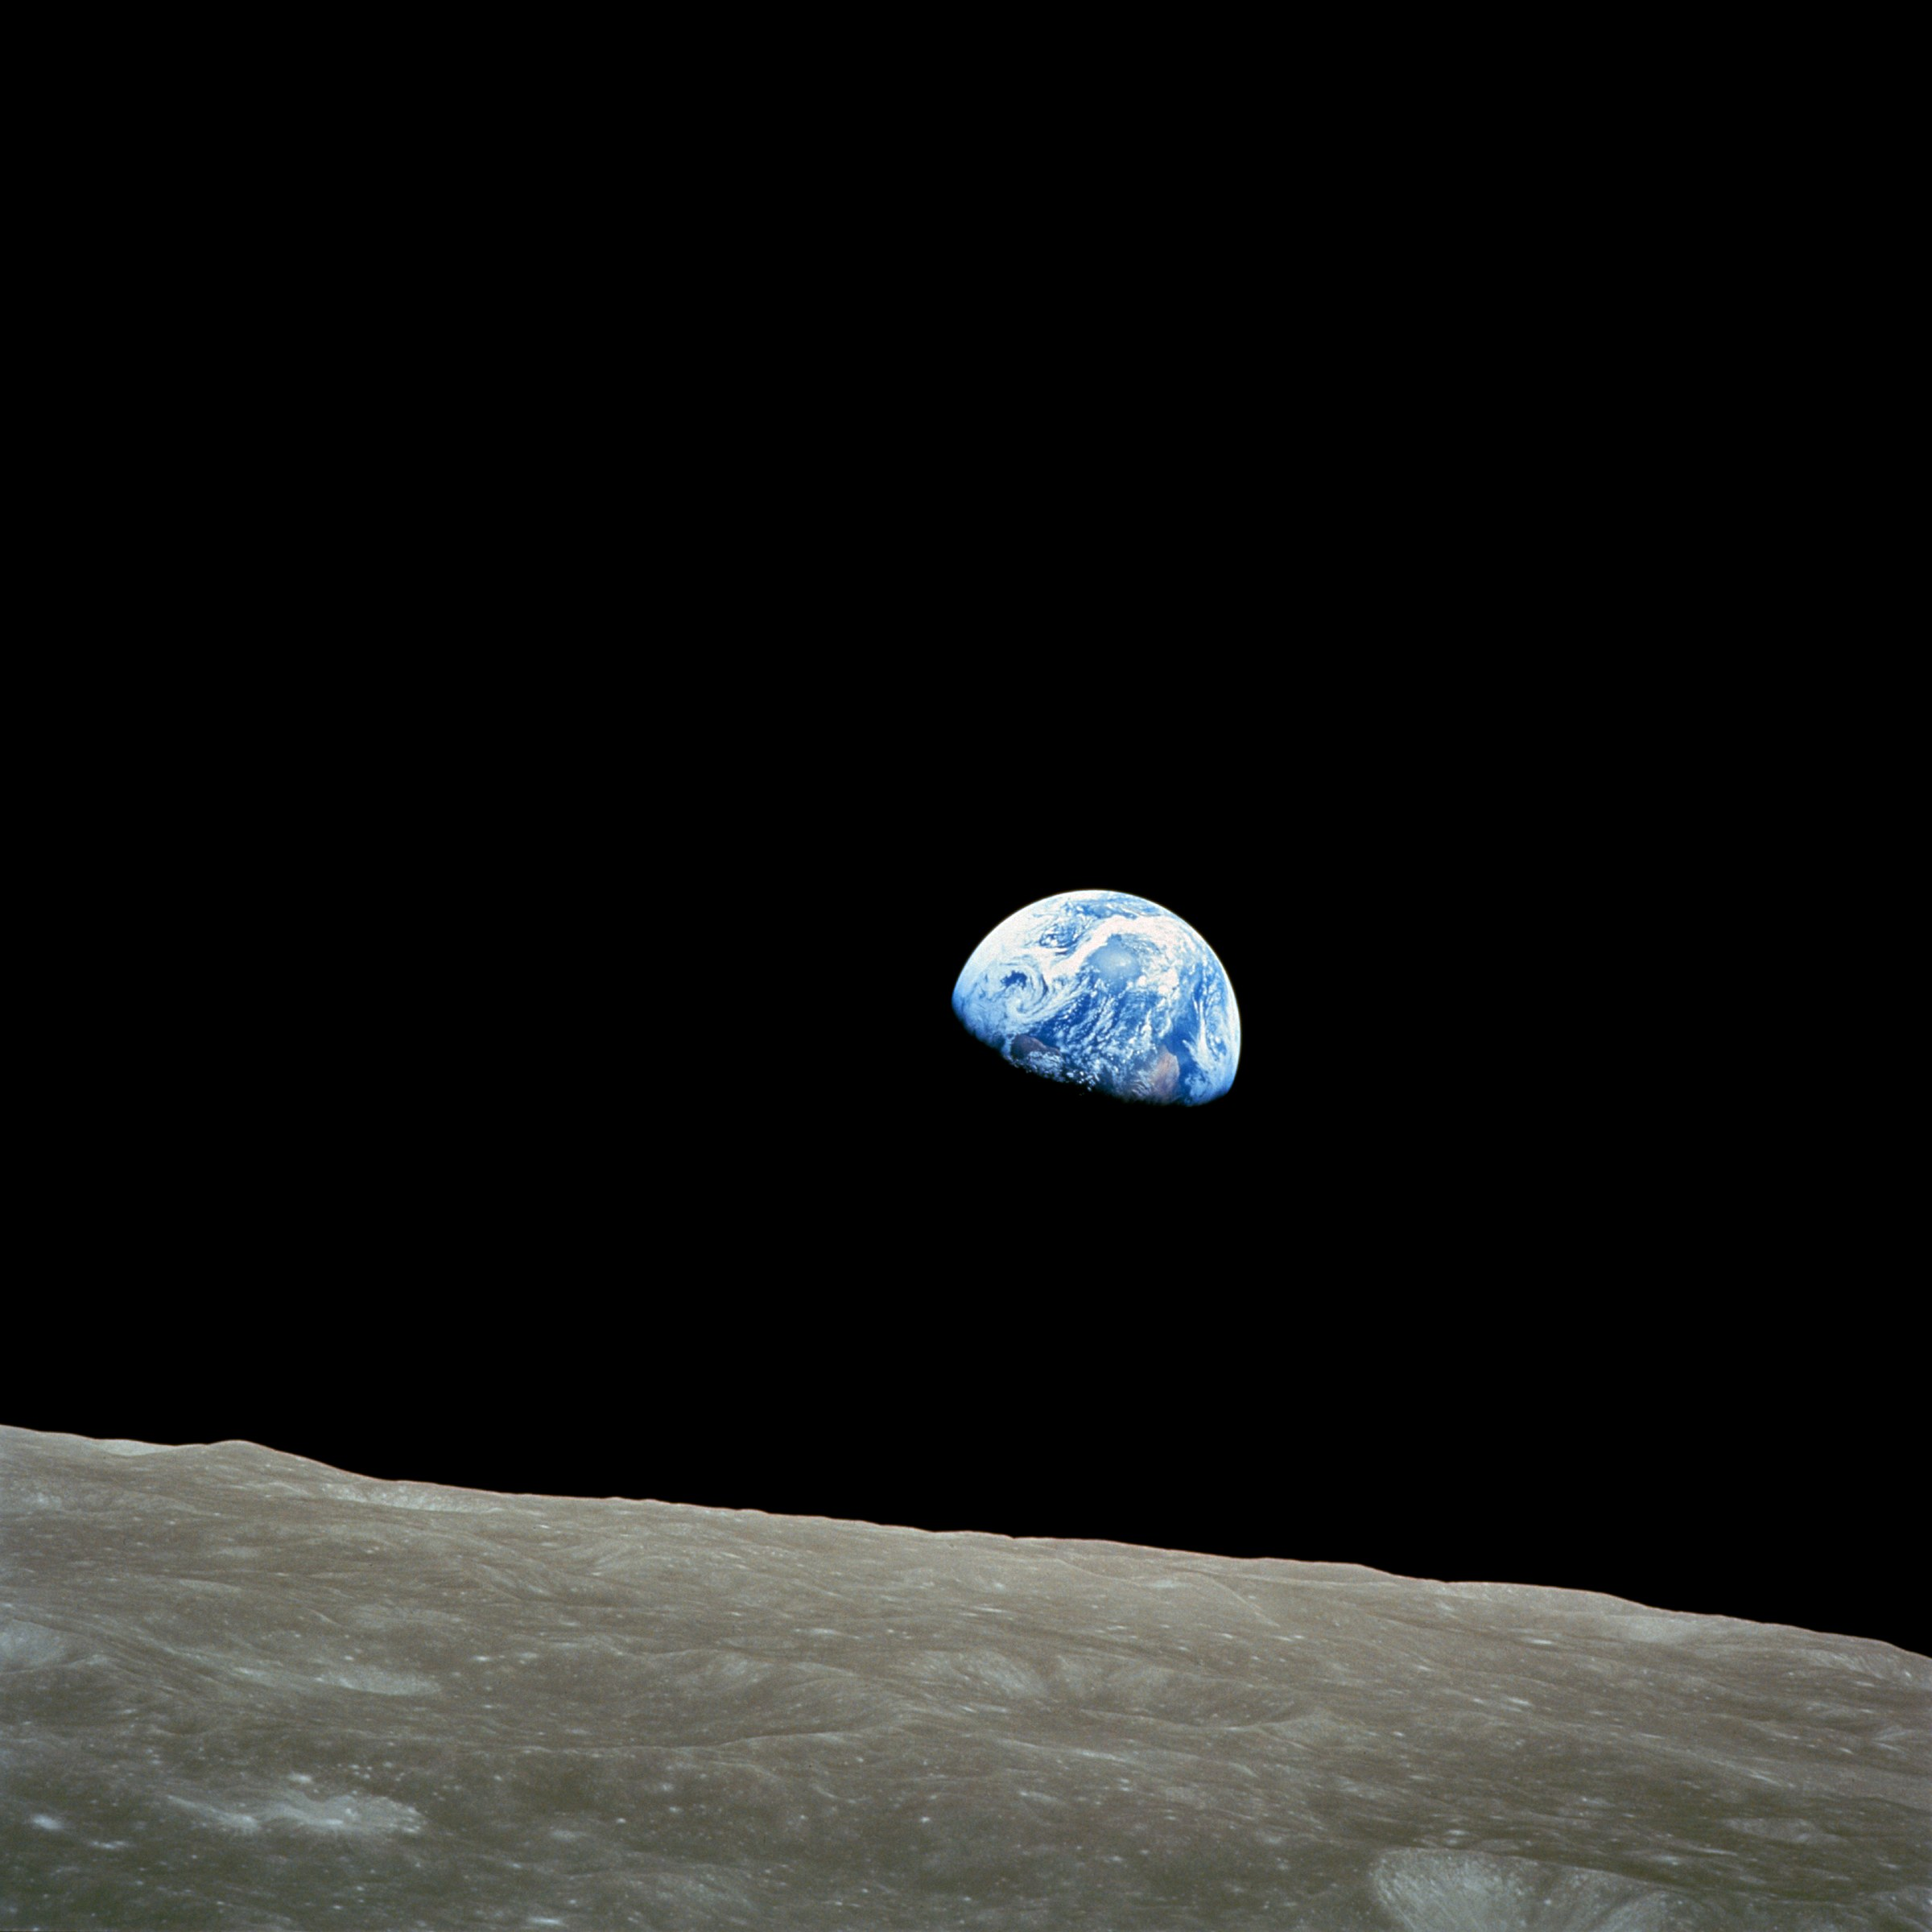
\includegraphics[width=0.6\textwidth]{earth-from-moon.jpg}

Earth seen from lunar orbit, {\it Apollo 8 (December 1968)}
\EC
}


\end{document}
